\documentclass[8pt,twoside]{report}

%%%%%%%%%%%%%%%%%%%%%%%%%%%%%%%%%%%%%%%%%%%%%%%%%%%%%%%%%%%%%%%%%%%%%%%%%%%%%

% Definitions for the title page
% Edit these to provide the correct information
% e.g. \newcommand{\reportauthor}{Timothy Kimber}

\newcommand{\reporttitle}{Autofaces}
\newcommand{\reportauthor}{Luka Milic}
\newcommand{\supervisor}{Sebastian Kaltzwang and Maja Pantic}
\newcommand{\degreetype}{Computing Science}

%%%%%%%%%%%%%%%%%%%%%%%%%%%%%%%%%%%%%%%%%%%%%%%%%%%%%%%%%%%%%%%%%%%%%%%%%%%%%
% load some definitions and default packages
%%%%%%%%%%%%%%%%%%%%%%%%%%%%%%%%%%%%%%%%%
% University Assignment Title Page 
% LaTeX Template
% Version 1.0 (27/12/12)
%
% This template has been downloaded from:
% http://www.LaTeXTemplates.com
%
% Original author:
% WikiBooks (http://en.wikibooks.org/wiki/LaTeX/Title_Creation)
%
% License:
% CC BY-NC-SA 3.0 (http://creativecommons.org/licenses/by-nc-sa/3.0/)
% 
%
%%%%%%%%%%%%%%%%%%%%%%%%%%%%%%%%%%%%%%%%%
%----------------------------------------------------------------------------------------
%	PACKAGES AND OTHER DOCUMENT CONFIGURATIONS
%----------------------------------------------------------------------------------------
\usepackage[a4paper,hmargin=2.8cm,vmargin=2.0cm,includeheadfoot]{geometry}
\usepackage{textpos}
\usepackage{natbib} % for bibliography
\usepackage{tabularx,longtable,multirow,subfigure,caption}%hangcaption
\usepackage{fncylab} %formatting of labels
\usepackage{fancyhdr} % page layout
\usepackage{url} % URLs
\usepackage[english]{babel}
\usepackage{amsmath}
\usepackage{graphicx}
\usepackage{dsfont}
\usepackage{epstopdf} % automatically replace .eps with .pdf in graphics
\usepackage{backref} % needed for citations
\usepackage{array}
\usepackage{latexsym}
\usepackage[pdftex,pagebackref,hypertexnames=false,colorlinks]{hyperref} % provide links in pdf

\hypersetup{pdftitle={},
  pdfsubject={}, 
  pdfauthor={},
  pdfkeywords={}, 
  pdfstartview=FitH,
  pdfpagemode={UseOutlines},% None, FullScreen, UseOutlines
  bookmarksnumbered=true, bookmarksopen=true, colorlinks,
    citecolor=black,%
    filecolor=black,%
    linkcolor=black,%
    urlcolor=black}

\usepackage[all]{hypcap}


%\usepackage{color}
%\usepackage[tight,ugly]{units}
%\usepackage{float}
%\usepackage{tcolorbox}
%\usepackage[colorinlistoftodos]{todonotes}
% \usepackage{ntheorem}
% \theoremstyle{break}
% \newtheorem{lemma}{Lemma}
% \newtheorem{theorem}{Theorem}
% \newtheorem{remark}{Remark}
% \newtheorem{definition}{Definition}
% \newtheorem{proof}{Proof}


%%% Default fonts
\renewcommand*{\rmdefault}{bch}
\renewcommand*{\ttdefault}{cmtt}



%%% Default settings (page layout)
\setlength{\parindent}{0em}  % indentation of paragraph

\setlength{\headheight}{14.5pt}
\pagestyle{fancy}
\renewcommand{\chaptermark}[1]{\markboth{\chaptername\ \thechapter.\ #1}{}} 

\fancyfoot[ER,OL]{\sffamily\textbf{\thepage}}%Page no. in the left on odd pages and on right on even pages
\fancyfoot[OC,EC]{\sffamily }
\renewcommand{\headrulewidth}{0.1pt}
\renewcommand{\footrulewidth}{0.1pt}
\captionsetup{margin=10pt,font=small,labelfont=bf}


%--- chapter heading

\def\@makechapterhead#1{%
  \vspace*{10\p@}%
  {\parindent \z@ \raggedright \sffamily
    \interlinepenalty\@M
    \Huge\bfseries \thechapter \space\space #1\par\nobreak
    \vskip 30\p@
  }}

%---chapter heading for \chapter*  
\def\@makeschapterhead#1{%
  \vspace*{10\p@}%
  {\parindent \z@ \raggedright
    \sffamily
    \interlinepenalty\@M
    \Huge \bfseries  #1\par\nobreak
    \vskip 30\p@
  }}

\allowdisplaybreaks

% load some macros
% Here, you can define your own macros. Some examples are given below.

\newcommand{\R}[0]{\mathds{R}} % real numbers
\newcommand{\Z}[0]{\mathds{Z}} % integers
\newcommand{\N}[0]{\mathds{N}} % natural numbers
\newcommand{\C}[0]{\mathds{C}} % complex numbers
\renewcommand{\vec}[1]{{\boldsymbol{{#1}}}} % vector
\newcommand{\mat}[1]{{\boldsymbol{{#1}}}} % matrix


\date{September 2016}
\begin{document}

% load title page
% Last modification: 2015-08-17 (Marc Deisenroth)
\begin{titlepage}

\newcommand{\HRule}{\rule{\linewidth}{0.5mm}} % Defines a new command for the horizontal lines, change thickness here


%----------------------------------------------------------------------------------------
%	LOGO SECTION
%----------------------------------------------------------------------------------------


\includegraphics[width = 4cm]{./figures/imperial}\\[0.5cm]

\center % Center remainder of the page

%----------------------------------------------------------------------------------------
%	HEADING SECTIONS
%----------------------------------------------------------------------------------------

\textsc{\Large Imperial College London}\\[0.5cm]
\textsc{\large Department of Computing}\\[0.5cm]

%----------------------------------------------------------------------------------------
%	TITLE SECTION
%----------------------------------------------------------------------------------------

\HRule \\[0.4cm]
{ \huge \bfseries \reporttitle}\\ % Title of your document
\HRule \\[1.5cm]

%----------------------------------------------------------------------------------------
%	AUTHOR SECTION
%----------------------------------------------------------------------------------------

\begin{minipage}{0.4\textwidth}
\begin{flushleft} \large
\emph{Author:}\\
\reportauthor % Your name
\end{flushleft}
\end{minipage}
~
\begin{minipage}{0.4\textwidth}
\begin{flushright} \large
\emph{Supervisor:} \\
\supervisor % Supervisor's Name
\end{flushright}
\end{minipage}\\[4cm]

% 
\includegraphics[width = 6cm]{./figures/imperial2}\\[0.5cm]

%----------------------------------------------------------------------------------------
%	FOOTER & DATE SECTION
%----------------------------------------------------------------------------------------
\vfill % Fill the rest of the page with whitespace
Submitted in partial fulfillment of the requirements for the MSc degree in
\degreetype~of Imperial College London\\[0.5cm]

\makeatletter
\@date
\makeatother


\end{titlepage}



% page numbering etc.
\pagenumbering{roman}
\clearpage{\pagestyle{empty}\cleardoublepage}
\setcounter{page}{1}
\pagestyle{fancy}

%%%%%%%%%%%%%%%%%%%%%%%%%%%%%%%%%%%%
\begin{abstract}
  Deep neural networks typically require large amounts of labelled data to make useful
  predictions, however in most domains this data is rare and mainly unlabelled.
  This project aims to incorporate that unlabelled data into a deep learning algorithm.
  A network with an autoencoder and classifier is proposed to be able to simultaneously
  learn from labelled and unlabelled data in a semi-supervised way. Detecting
  facial actions units is the chosen domain to benchmark this approach, with
  the DISFA dataset being used for preliminary experiments.
\end{abstract}

\cleardoublepage
%%%%%%%%%%%%%%%%%%%%%%%%%%%%%%%%%%%%
\section*{Acknowledgements}
Sebastian - Doing face detection on the DISFA images.

\clearpage{\pagestyle{empty}\cleardoublepage}

%%%%%%%%%%%%%%%%%%%%%%%%%%%%%%%%%%%%
%--- table of contents
\fancyhead[RE,LO]{\sffamily {Table of Contents}}
\tableofcontents


\clearpage{\pagestyle{empty}\cleardoublepage}
\pagenumbering{arabic}
\setcounter{page}{1}
\fancyhead[LE,RO]{\slshape \rightmark}
\fancyhead[LO,RE]{\slshape \leftmark}

\chapter{Introduction}
  talk about self-reported pain and intensity estimation
  why didn't I do any intensity estimation stuff?
  Regression is difficult??? Classification is a different thing.
  take about the fact that you are doing one frame and a time and
  other methods might be better becuse they can do sequences.
  \section{Problem Space}
    The human face is most likely one of the most researched objects in image analysis
    and computer vision \cite{S.ZafeiriouA.PapaioannouI.KotsiaM.A.Nicolaou}.
    It has wide ranging applications from Human
    Computer Interaction (expression recognition) to law enforcement (face recognition).
    Its study necessitates the development of a wide range of machine
    learning and computer vision research.

    Facial Action Unit detection FAU \cite{Corneanu2016} is chosen in this work due
    to it's popularity and available benchmarks.
    The Facial Action Coding System (FACS) developed by Ekman and Friesen,
    provides a systematic way to study any kind of facial expression,
    by representing them as a combination of individual facial muscle actions
    known as Action Units (AU). Automating the process of detecting AUs is difficult
    because they have non-linear interactions and often occur in very low intensities.

    There exist many datasets containing images and videos of faces and it is a general
    observation that unlabelled images are far more abundant than labelled ones.
    In particular in the areas of expression recognition where painstaking work
    must be carried out to obtain the ground truth expressions for an image or set of
    frames in a video. This situation is one of the motivations for this project.

    \begin{figure}
     \centering
     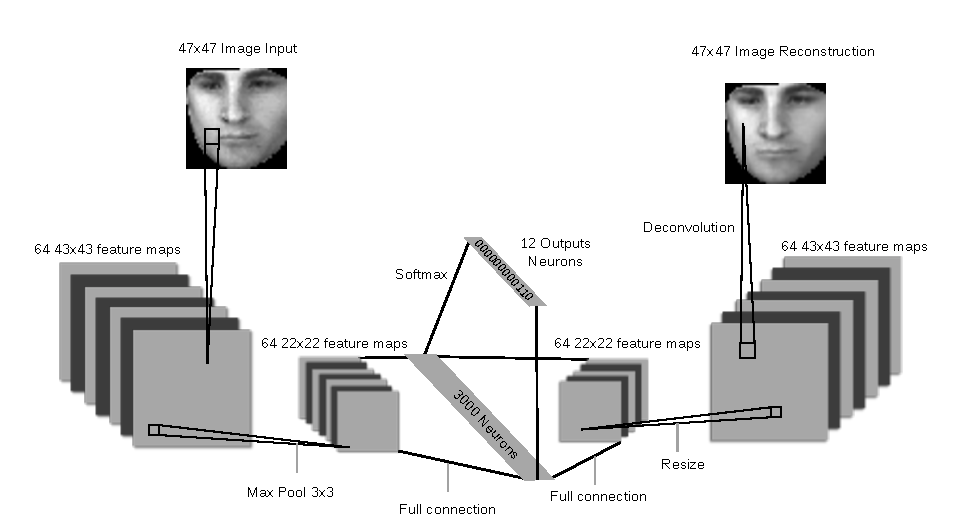
\includegraphics[width=\textwidth]{illustrations/aec_network.pdf}
     \captionof{figure}{General structure of the proposed network. Each rectangle
     represents many layers of neurons and the thin lines represent connections between layers.}
    \end{figure}

    Deep learning is emerging as a powerful tool in modelling a wide range of patterns
    in data, it has been applied to the problem of FAU a number of times and achieved
    good classification rates. One complication which arises when using Deep Neural
    Networks DNNs to classify AUs is that many frames are unlabelled (have neutral expressions)
    and hence the standard supervised DNN do not make good use of this information.
    This project aims to investigate how an autoencoder could be combined with the
    already established deep learning methods related to FAU in order to improve the performance
    of these techniques and better leverage unlabelled data. This unlabelled data may
    come from within the standard AU datasets or from larger databases of faces.
    The DISFA dataset is chosen for initial experiments.
  \section{Potential Applications}
  \section{Contributions}
  \section{Thesis Outline}

\chapter{Background}

\section{Databases for FAU estimation}
Relevant for this work is a awareness of datasets which exist and which may be useful
for experiments. Here is a list of some which should be used in order to allow
this project to be comparable to work in the literature:

\begin{itemize}
    \item The DISFA database \cite{disfa}, which contains 27 subjects whose spontaneous
          facial expressions were captured in controlled recording conditions.
    \item CK+ \cite{Lucey2010} containing 123 subjects recorded with faces in strictly front positions.
    \item FERA 2015 BP4D-Spontaneous Dataset \cite{Valstar}:
          containing 41 subjects and 34 AUs, the subjects were young adults who
          spontaneously generated emotional responses to stimulus tasks.
\end{itemize}

This is just a small selection, however is it representative of the types of
datasets available. Each frame of the videos has a label which describes which AUs are
present and their intensity. Hence two distinct problems can be tackled here, intensity
estimation and classification, this work follows the classification route however
intensity estimation should also be possible with a few minor modifications.

A key challenge with these datasets is that they often have very unbalanced and
sparse labels as shown in figure \ref{disfastats}. This calls for methods
to balance training samples with respect to this imbalance and is the
motivation for using some unsupervised learning techniques, in order to extract information
from the unlabelled data.

A further two datasets are the TFD and SEMAINE, these do not contain AUs but often crop up in the
literature:
\begin{itemize}
     \item TFD \cite{tfd} Toronto Face Dataset
     \item The SEMAINE \cite{semaine} corpus which contains recordings
           of people interacting with a Sensitive Artificial Listener (SAL) in controlled conditions.
\end{itemize}

\section{The DISFA dataset} \label{disfa_list}
The Denver Intensity of Spontaneous Facial Action Dataset (DISFA)
Of central interest to the project is the DISFA dataset \cite{disfa}, it is a set
of videos of people watching 9 short clips from youtube which try to span a range
of emotions such as emotions happiness, surprise, fear, disgust and sadness. Included
are 27 subjects with 12 AUs.

Each frame in each subject video has a label which says how much of each AU is present on
a scale of 0-5, the distribution of intensities is shown in table \ref{compau}.

A challenge of the DISFA dataset is that it has many frames which are unlabelled, this is demonstrated
per subject in figure \ref{disfastats}. Many of the subjects have over 40\% of their frames unlabelled
, one outlier has over 75\% unlabelled.

\begin{table}[h!]
\centering

\begin{tabular}{lllllll}
\hline
Intensity & 0      & 1     & 2     & 3     & 4    & 5    \\ \hline
AU1       & 112286 & 2272  & 1749  & 2809  & 1393 & 555  \\
AU2       & 99165  & 1720  & 934   & 3505  & 836  & 369  \\
AU4       & 106160 & 4661  & 7636  & 6586  & 4328 & 1383 \\
AU5       & 99015  & 1579  & 719   & 293   & 104  & 34   \\
AU6       & 106425 & 9157  & 5986  & 3599  & 601  & 141  \\
AU9       & 99458  & 1659  & 2035  & 3045  & 316  & 77   \\
AU12      & 99987  & 13943 & 6869  & 7233  & 2550 & 172  \\
AU15      & 108358 & 5180  & 1618  & 1017  & 47   & 0    \\
AU17      & 117824 & 6342  & 4184  & 2281  & 112  & 11   \\
AU20      & 121377 & 1591  & 1608  & 1305  & 28   & 0    \\
AU25      & 84721  & 9805  & 13935 & 15674 & 5580 & 1039 \\
AU26      & 105778 & 13443 & 7473  & 3529  & 314  & 217  \\ \hline
\end{tabular}
\caption{A comparison of the number of occurrences of each intensity for each AU in the DISFA dataset} \label{compau}
\end{table}


\begin{figure}[h!]
  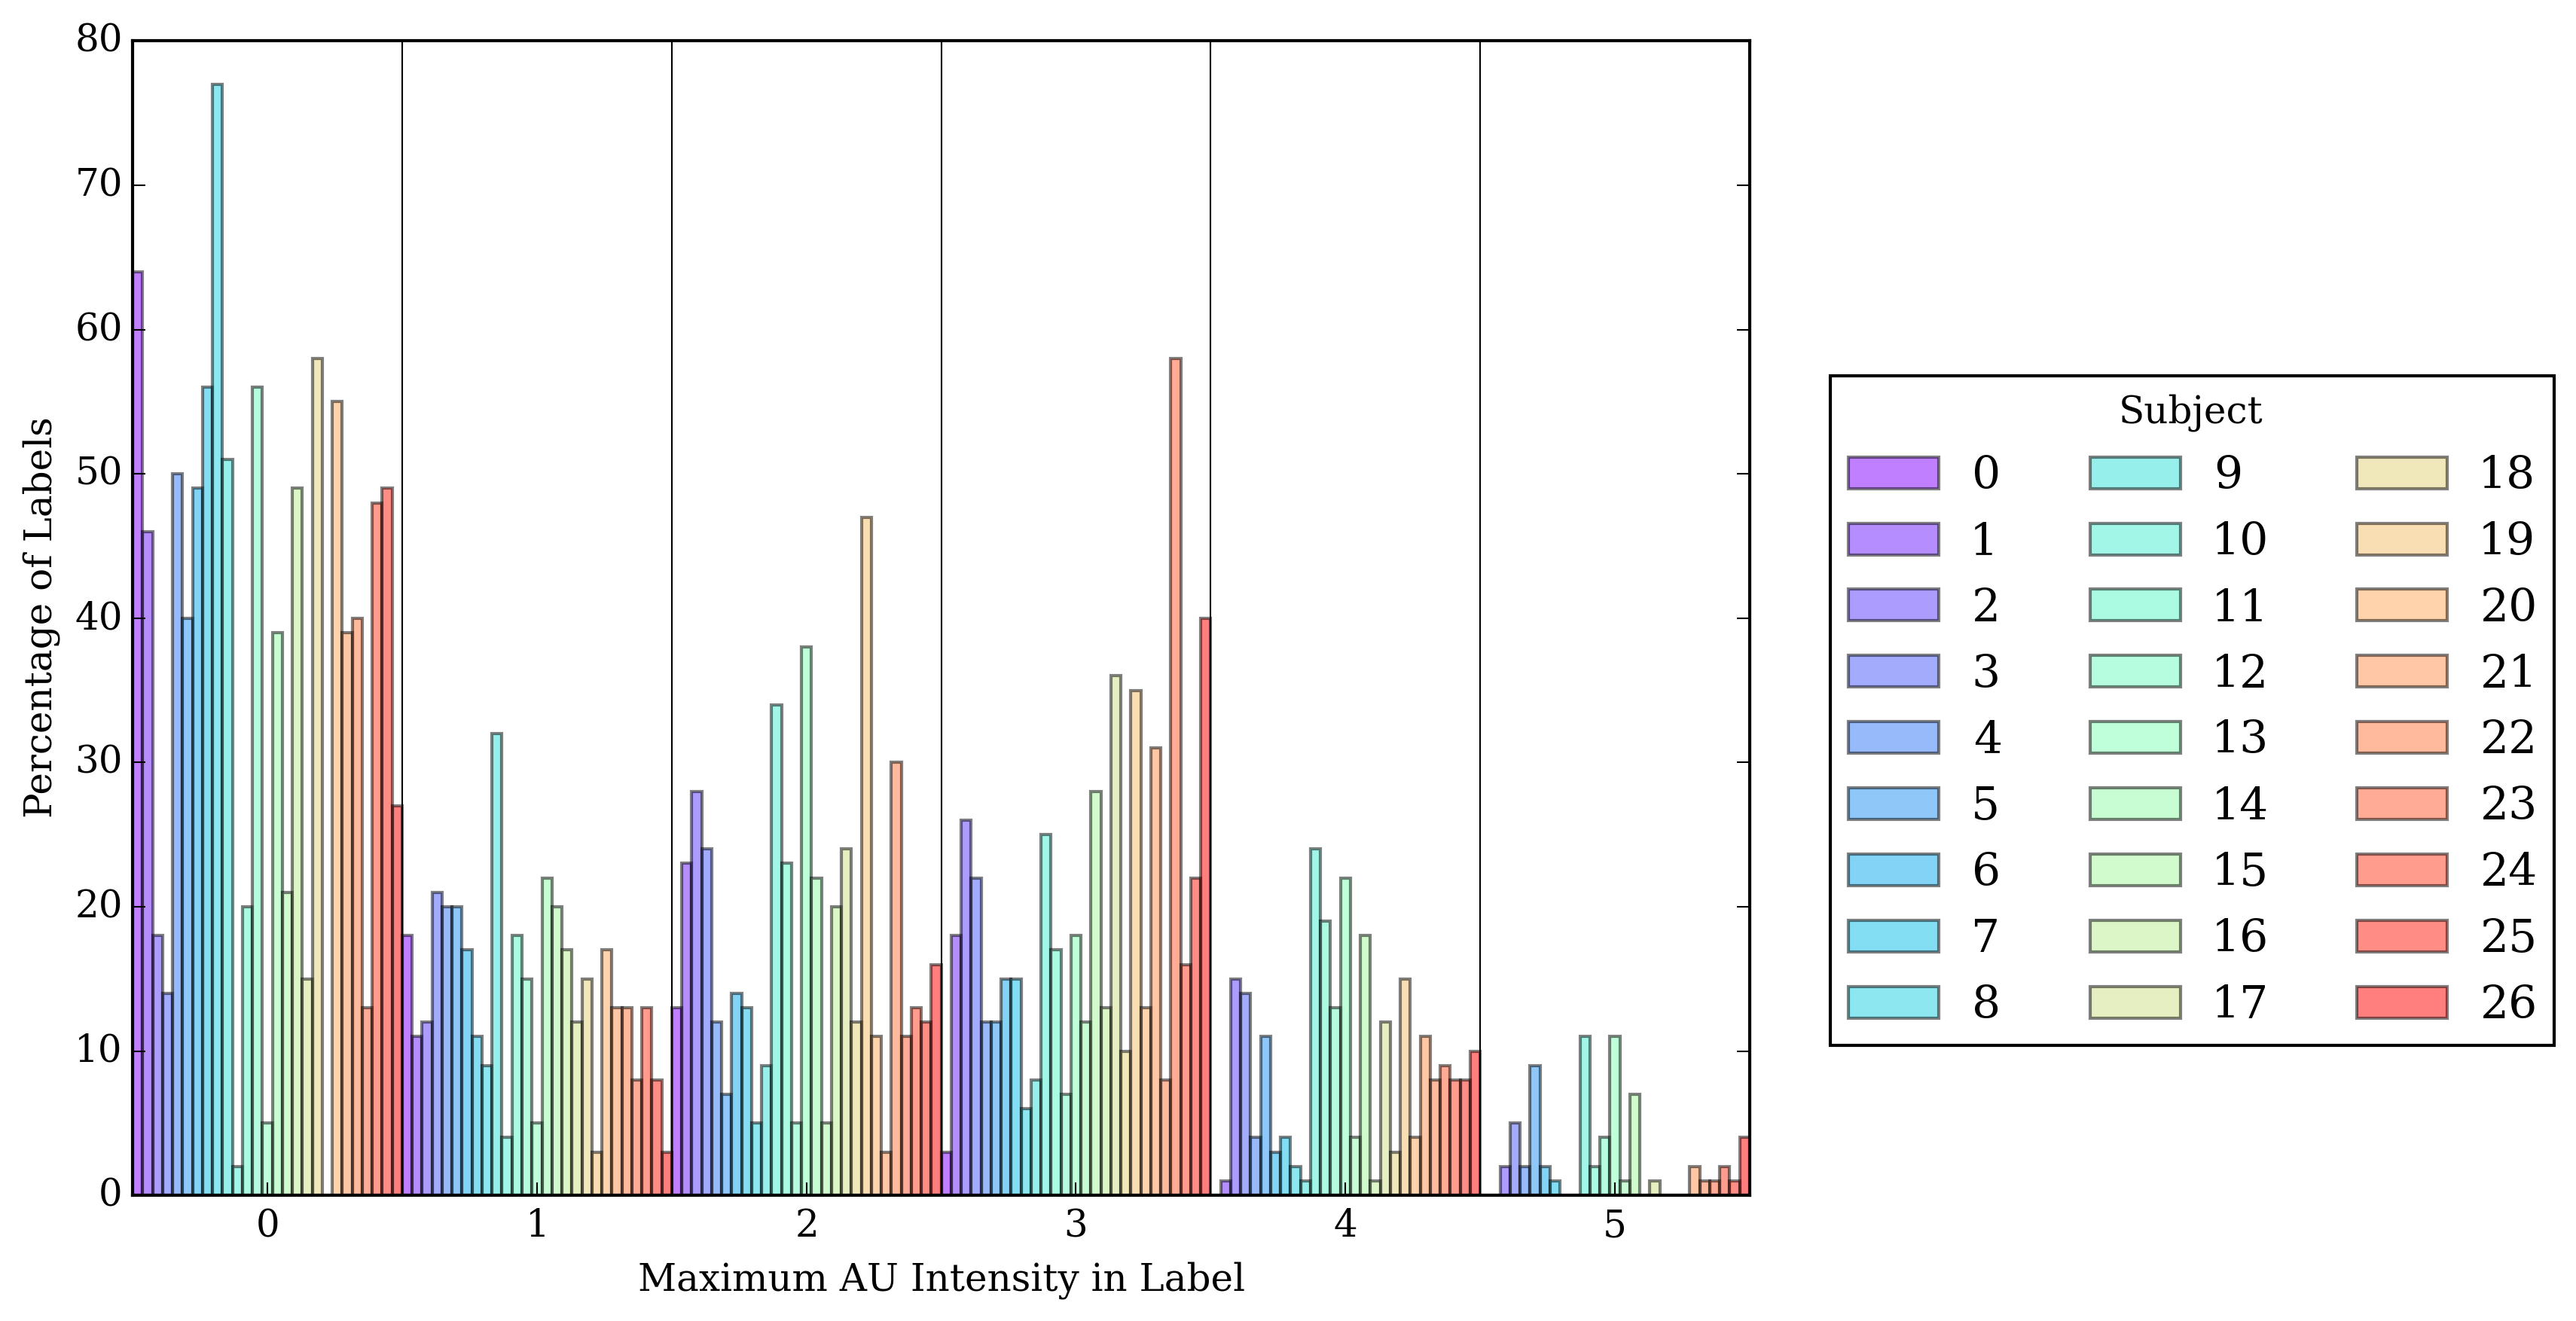
\includegraphics[width=\textwidth]{../graphs/maximum_label_intensity_disfa.pdf}
  \caption{DISFA dataset: This graph shows what the maximum value in each label is in the DISFA dataset per subject. This
  is done to illustrate the number of labels which contain very little information
  and pose an issue for a typical neural network structure.}\label{disfastats}
\end{figure}
\newpage

\section{Deep learning approaches to FAU detection}
It has been shown that deep neural networks containing convolutional, max pooling,
dropout and fully connected layers can effectively learn how to classify AUs in
a selection of datasets \cite{Gudi2015,Ghosh2015,dodeeplearn}. For theoretical information
about these networks see Chapter \ref{chapter:deep} These
works only include networks which ignore the temporal structure of the data,
other architectures do incorporate this \cite{emonet,Jaiswal2016}.
%
%
%
\subsection*{Comparison of networks in Table \ref{compnet}}
Network \cite{Ghosh2015} (Ghosh et al.) was trained on CK+, DISFA and BP4D datasets.
A key result of this paper was that they achieved good generalisation between datasets
with classifications accuracies between 60\% and 80\% for these generalisation experiments.
A feature particular to this network was that after the softmax layer, which assigns probabilities
to each AU it uses QDA (Quadratic Discriminant Analysis) \cite{precogbook} to
make predictions about whether AUs are present. A point of interest is also that
mean face normalisation is done per subject and then all for all subjects.

Network \cite{Gudi2015} (Amogh Gudi et al.) was trained on BP4D and SEMAINE
datasets achieving an average F1 score of 0.52 and 0.34 respectively. This paper
uses minimal preprocessing hence is a good example of how CNNs can learn features
with little feature engineering.

Network \cite{dodeeplearn} (Pooya Khorrami et al.) was trained on TFD and CK+,
this got average accuracies of 89.9\% and 98.3\% respectively in detecting emotions. This
is therefore not directly comparable, but they do explore connecting it with AUs.
An interesting point about this work is that they could stimulate activations in the convolutional
layers and directly see that the network had learned different facial actions demonstrating the
power of these networks.

Network \cite{Jaiswal2016} (Shashank Jaiswal et al.) was trained on SEMAINE and
BP4D achieving an overall weighted F1 score of 0.54. Which is on average higher
than network \cite{Gudi2015} as claimed in the paper. This paper includes a lot more
prior knowledge than the others, firstly it uses a BLSTM to incorporate temporal structure
and it defines multiple input streams from each facial region, allowing the convolutional
filters to become more specialised. This is the only paper where they say they use
two outputs for each AU so that the softmax creates a probability distribution for
each AU and not for all of them at once.

It should be noted that it is difficult to compare the performance between these
networks as they all use different evaluation scores as shown in table \ref{compscore}.

\begin{table}[h!]
\centering
{\footnotesize
\begin{tabular}{|lllllllll|}
\hline
Network                      & \multicolumn{2}{c}{Ghosh et. al\cite{Ghosh2015}}                         & \multicolumn{2}{c}{Gudi et. al.\cite{Gudi2015}}                            & \multicolumn{2}{c}{Khorrami et. al.\cite{dodeeplearn}}                          & \multicolumn{2}{c|}{Jaiswal et. al.\cite{Jaiswal2016}}   \\ \hline
\multicolumn{1}{|l|}{Element} & Type     & \multicolumn{1}{l|}{Dimensions}                    & Type     & \multicolumn{1}{l|}{Dimensions}                      & Type          & \multicolumn{1}{l|}{Dimensions}                  & Type      & Dimensions                     \\ \hline
\multicolumn{1}{|l|}{x}       &          & \multicolumn{1}{l|}{$40\times40\times1$}           &          & \multicolumn{1}{l|}{$48\times 48\times1$}            &               & \multicolumn{1}{l|}{$96\times96\times1$}         &           & $?\times?\times1$              \\ \hline
\multicolumn{1}{|l|}{$L_1$}   & conv 1   & \multicolumn{1}{l|}{$12\times 12\times1\times 70$} & conv 1   & \multicolumn{1}{l|}{$5\times 5\times1\times64$}      & conv 1        & \multicolumn{1}{l|}{$5\times5\times1\times64$}   & conv 1*   & $5\times5\times(2n+1)\times32$ \\
\multicolumn{1}{|l|}{$y_1$}   &          & \multicolumn{1}{l|}{$29\times29\times70$}          &          & \multicolumn{1}{l|}{$44\times44\times64$}            &               & \multicolumn{1}{l|}{$92\times92\times64$}        &           & $?\times?\times32$             \\ \hline
\multicolumn{1}{|l|}{$L_2$}   & max pool & \multicolumn{1}{l|}{$2\times 2$}                   & max pool & \multicolumn{1}{l|}{$3\times3$ (stride 2)}           & max pool      & \multicolumn{1}{l|}{$2\times2$}                  & max pool*  & $3\times3$                    \\
\multicolumn{1}{|l|}{$y_2$}   &          & \multicolumn{1}{l|}{$15\times15\times 70$}         &          & \multicolumn{1}{l|}{$22\times 22\times64$}           &               & \multicolumn{1}{l|}{$46\times46\times64$}        &           & $?\times?\times32$             \\ \hline
\multicolumn{1}{|l|}{$L_3$}   & conv 2   & \multicolumn{1}{l|}{$4\times 4\times70\times 10$}  & conv 2   & \multicolumn{1}{l|}{$5 \times 5 \times 64\times64$}  & conv 2        & \multicolumn{1}{l|}{$5\times5\times64\times128$} & conv 2    & $5\times5\times32\times64$     \\
\multicolumn{1}{|l|}{$y_3$}   &          & \multicolumn{1}{l|}{$12\times 12 \times 10$}       &          & \multicolumn{1}{l|}{$18 \times 18\times64$}          &               & \multicolumn{1}{l|}{$42\times42\times128$}       &           & $?\times?\times64$             \\ \hline
\multicolumn{1}{|l|}{$L_4$}   & max pool & \multicolumn{1}{l|}{$2\times 2$}                   & conv 3   & \multicolumn{1}{l|}{$4\times 4 \times64 \times 128$} & max pool      & \multicolumn{1}{l|}{$2\times2$}                  & conv 3    & $5\times5\times64\times64$     \\
\multicolumn{1}{|l|}{$y_4$}   &          & \multicolumn{1}{l|}{$6\times 6 \times 12$}         &          & \multicolumn{1}{l|}{$15\times15\times128$}           &               & \multicolumn{1}{l|}{$21\times21\times128$}       &           & $?\times?\times64$             \\ \hline
\multicolumn{1}{|l|}{$L_5$}   & fc       & \multicolumn{1}{l|}{$500$}                         & fc       & \multicolumn{1}{l|}{$3072$}                          & conv 3        & \multicolumn{1}{l|}{$5\times5\times1\times256$}  & conv 3    & $4\times4\times64\times128$    \\
\multicolumn{1}{|l|}{$y_5$}   &          & \multicolumn{1}{l|}{$500$}                         &          & \multicolumn{1}{l|}{$3072$}                          &               & \multicolumn{1}{l|}{$17\times17\times256$}       &           & $?\times?\times128$            \\ \hline
\multicolumn{1}{|l|}{$L_6$}   & fc       & \multicolumn{1}{l|}{$100$}                         & softmax  & \multicolumn{1}{l|}{$12$}                            & quadrant pool & \multicolumn{1}{l|}{}                            & fc        & $3072$                         \\
\multicolumn{1}{|l|}{$y_6$}   &          & \multicolumn{1}{l|}{$100$}                         &          & \multicolumn{1}{l|}{$12$}                            &               & \multicolumn{1}{l|}{$4\times4\times256$}         &           & $3072$                         \\ \hline
\multicolumn{1}{|l|}{$L_7$}   & softmax  & \multicolumn{1}{l|}{$12$}                          &          & \multicolumn{1}{l|}{}                                & fc            & \multicolumn{1}{l|}{$300$}                       & softmax   & $2N_{C}$                       \\
\multicolumn{1}{|l|}{$y_7$}   &          & \multicolumn{1}{l|}{$12$}                          &          & \multicolumn{1}{l|}{}                                &               & \multicolumn{1}{l|}{$300$}                       &           & $2N_{C}$                       \\ \hline
\multicolumn{1}{|l|}{$L_8$}   & QDA      & \multicolumn{1}{l|}{}                              &          & \multicolumn{1}{l|}{}                                & softmax       & \multicolumn{1}{l|}{$8$}                         & BLSTM     &                                \\
\multicolumn{1}{|l|}{$y_8$}   &          & \multicolumn{1}{l|}{}                              &          & \multicolumn{1}{l|}{}                                &               & \multicolumn{1}{l|}{$8$}                         &           &                                \\ \hline
\end{tabular}

\caption{A comparison of network architectures from the literature, all networks
use RELUs as their activation functions apart from in the final layer where it is
typical to use a softmax. $x$ denotes the input image, $L_i$ denotes the $i$th layer and $y_i$ denotes the output of the $i$th layer.
$N_{C}$ is the number of classes.
The question marks signify the dimensions of input images are variable as it depends on the input stream. fc is for fully connected and
conv is for convolutional layer. QDA is Quadratic Discriminant Analysis and BLSTM is for Bidirectional Long Short-Term Memory neural
networks.
\newline
*These layers are per input stream} \label{compnet}

}
\end{table}

\begin{table}[h!]
\centering

\begin{tabular}{lcccc}
\hline
Score    & \multicolumn{1}{l}{Ghosh et. al\cite{Ghosh2015}} & \multicolumn{1}{l}{Gudi et. al.\cite{Gudi2015}} & \multicolumn{1}{l}{Khorrami et. al.\cite{dodeeplearn}} & \multicolumn{1}{l}{Jaiswal et. al.\cite{Jaiswal2016}} \\ \hline
Accuracy & \checkmark                                       &                                                 & \checkmark                                             &                                             \\
F1       &                                                  & \checkmark                                      &                                                        & \checkmark                                  \\
AUC      &                                                  &                                                 &                                                        &                                             \\
2AFC     & \checkmark                                       & \checkmark                                      &                                                        &                                             \\ \hline
\end{tabular}
\caption{A comparison of which evaluation methods were used in the relevant papers.} \label{compscore}
\end{table}

\begin{table}[h!]
\centering

\begin{tabular}{lcccc}
\hline
Dataset    & \multicolumn{1}{l}{Ghosh et. al\cite{Ghosh2015}} & \multicolumn{1}{l}{Gudi et. al.\cite{Gudi2015}} & \multicolumn{1}{l}{Khorrami et. al.\cite{dodeeplearn}} & \multicolumn{1}{l}{Jaiswal et. al.\cite{Jaiswal2016}} \\ \hline
CK+      & \checkmark                            &                                      &                                         & \checkmark                              \\
DISFA    & \checkmark                            &                                      &                                         &                                         \\
SEMAINE* &                                       & \checkmark                           & \checkmark                              &                                         \\
BP4D*    & \checkmark                            & \checkmark                           & \checkmark                              &                                         \\
TFD      &                                       &                                      &                                         & \checkmark                              \\ \hline
\end{tabular}
\caption{A comparison of which datasets were used in the relevant papers.} \label{compdat}
\end{table}


%
%
%

\chapter{Deep Learning Background} \label{chapter:deep}
  \section{Introduction}
    pass
  \section{Model Components}
    \subsection{Artificial Neural Networks}
  An artificial neuron is a function which takes in a vector of inputs, computes their
  weighted sum and applies a non-linearity as follows:
  \begin{equation}
    a(\mathbf{x}) = \sigma \left ( \sum_{i=1}^N w_ix_i + b \right )
  \end{equation}
  Here $\sigma$ is a scalar function, $w_i$ is a scalar weight and $b$ is its bias. $N$ is the size of the input and weight vector.
  These neurons can be combined into layered networks to construct artificial neural networks.
  The weights $w$ can then be rewritten as matrices $\mathbf{W}$ which define how
  activations from one layer are transferred to the next\footnote{Note: when a vector
  is put into a scalar function it is assumed that it acts on each element of
  the vector. The only exception is with the softmax.}.
  \begin{equation}
    \mathbf{a}(\mathbf{x}) = \mathbf{\sigma} \left ( \mathbf{W}\mathbf{x} + \mathbf{b} \right ) \label{eq:softmax}
  \end{equation}

  Popular activation functions include:
  \begin{multicols}{2}


    \begin{equation}
      \text{The sigmoid:}\quad
      \sigma (x) = \frac{1}{1-e^{-x}} \label{eq:sigmoid}
    \end{equation}


    \begin{equation}
      \text{The ReLU:}\quad
      \sigma(x) =
      \begin{cases}
        x & x\geq 0 \\
        0 & x < 0
      \end{cases}
    \end{equation}


    \begin{equation}
      \text{Hyperbolic tan:}\quad
      \sigma(x)=\frac{e^x - e^{-x}}{e^x + e^{-x}}
    \end{equation}


    \begin{equation}
      \text{The softmax:}\quad
      \sigma(\mathbf{x})_j = \frac{e^{x_j}}{\sum_i e^{x_i}}
    \end{equation}


  \end{multicols}

  \begin{figure} \label{disfagraph}
    \center
    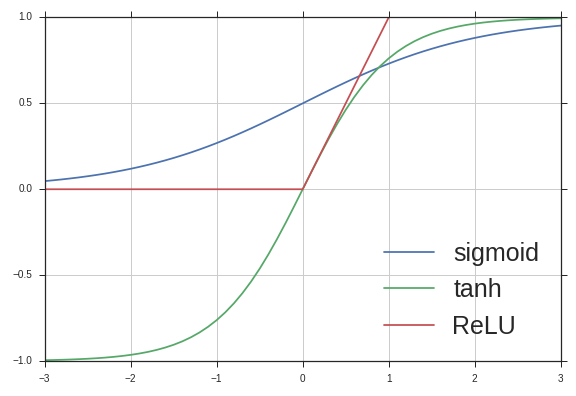
\includegraphics[width=.5\textwidth]{../graphs/actfuncs.pdf}
    \caption{Comparison of common activation functions for neural networks}
  \end{figure}



  An $N$ layer network can
  then be thought of as a function with a recursive structure (these are also known as fully connected layers):
  \begin{equation}
    \mathbf{y} = \mathbf{a}_{N}(\mathbf{a}_{l-1}(...\mathbf{a}_1(\mathbf{x})...))
  \end{equation}
  Now assuming there exists a set of $\tilde{\mathbf{x}}$ and $\tilde{\mathbf{y}}$ which make
  up a training data set, these could be sets of images and labels, then a cost function
  to optimise can be defined:
  \begin{equation}
    J(\tilde{\mathbf{x}},\tilde{\mathbf{y}}) = \frac{1}{N}\left |\mathbf{y}(\tilde{\mathbf{x}})-\tilde{\mathbf{y}}\right | ^2
  \end{equation}
  this is called the least mean squared error, another popular cost function is
  the cross entropy:
  \begin{equation}
    J(\tilde{\mathbf{x}},\tilde{\mathbf{y}}) = -\frac{1}{N}\tilde{\mathbf{y}}\cdot\log(\mathbf{y}(\tilde{\mathbf{x}}))
  \end{equation}

  The derivative of these cost functions can then be computed in order to minimise it.
  The simplest way is to do this is per training example, however stochastic gradient
  descent\cite{Amari1993} has emerged as a superior method. Simply put it computes the gradient with respect
  to many randomly drawn samples, it has the advantage of following a smoother path
  towards the local minimum.
  \subsection{Convolutional Layers}
  A convolutional layer is a generalisation of simple fully connected layers described
  above. It consists of a set of $K$ filters of size $m\times m$, which are applied to the input to produce
  a set of $K$ outputs. The filters are applied with a 2D convolution.


  To describe them, firstly assume that any vector described in the previous section
  can also be rewritten as a matrix, i.e $\mathbf{x} \in \mathbb{R}^{n}
  \rightarrow \mathbf{x} \in \mathbb{R}^{N \times M} \quad NM=n$, in practice this is made
  easy by using numbers which factorise well.

  Then the following equation describes the output of a convolutional layer:
  \begin{equation} \label{CNN}
    \mathbf{a}(\mathbf{x})_{ijk} = \sigma \left ( \sum_{a=0}^{m-1}\sum_{b=0}^{m-1}(w_{abk}x_{(i+a)(j+b)k}) + b_k \right )
  \end{equation}
  Here $i,j$  denote row, column indices for the matrix (image) $\mathbf{x}$, $k$ is the filter index, $w_{abk}$
  gives the filter element and $b_k$ is the bias for that filter. This is done for all $K$ filters.

  One issue is how to deal with indices which are out of bounds, SAME padding can be used which sets out of bounds
  elements to zero and so preserves the image size or VALID can be used, this keeps the filter within the bounds of the
  image and hence the output is of a smaller dimension. Lastly a stride greater than 1 can be incorporated into equation
  \ref{CNN} meaning that $\mathbf{a}$ is only computed for a fraction of indices $i,j$.
  % \begin{equation}
  % 	C : \mathbb{R}^{n\times m \times p \times l} \rightarrow \mathbb{R}^{N\times M \times l \times K}
  % \end{equation}
  %con%
  \subsection{Max Pooling Layers}
  A max pooling layer simply splits its input into a set of sections and extracts
  the highest value from each. It is a simple but effective method to down sample
  an image, it helps to keep the computational overhead of these algorithms
  down. However a recent trend \cite{Springenberg2015} has emerged where max pooling
  layers are not used, instead a convolutional layer with a large stride accomplishes
  the same amount of down-sampling.
    \subsection{Cost Functions}
      pass
    \subsection{Training algorithms}
      pass
      \subsubsection{Gradient Descent}
        pass
      \subsubsection{Stochastic Gradient Descent}
        pass
      \subsubsection{Adam}
        pass
      \subsubsection{Comparison}
        pass
    \subsection{Regularisers}
      pass
    \subsection{Dropout Layers} \label{sec:dropout}
      A layer with dropout applied to it randomly turns neurons off, making it more
      difficult for the network to overfit data. There is a dropout probability
      which determines how often neurons are disabled, it is typically under 20\%
    \subsection{Autoencoders}
      An autoencoder is at its bare minimum a artificial neural network which tries
      to reproduce its input as accurately as possible. So the cost function for the mean squared error becomes:

      \begin{equation} \label{eq:autoencoder_cost}
        J(\tilde{\mathbf{x}},\tilde{\mathbf{y}}) = \frac{1}{N}\left |\mathbf{y}(\tilde{\mathbf{x}})-\tilde{\mathbf{x}}\right | ^2
      \end{equation}

      Constraints are
      placed on the network so that it has to learn to compress the input, the following
      are popular constraints that may be used:
      \begin{itemize}
        \item Few neurons in the hidden layers
        \item Sparsity: the average activation of the neurons can be kept under a
        threshold, typically a small value close to zero \cite{autong}
        \item Noise may be added to the input, this makes the network more likely
        to learn general features.
      \end{itemize}
      Lastly there are Variational Autoencoders which combine ideas from Bayesian inference
      to create networks which can not only reconstruct their input but also act as a
      distribution which can be sampled from, allowing for the generation of new samples \cite{Kingma2013}.

    \subsection{Stacked Autoencoder}
      A stacked autoencoder is typically used for pre-training a network for a classification task.
      Instead of training the whole structure at once, each layer is trained as the last hidden
      layer of some temporary autoencoder. It has been shown that this can improve classification performance \cite{stacks}.
    \subsection{Convolutional Autoencoder}
      A convolutional autoencoder works in the same way as a standard autoencoder, however
      undoing the max pooling presents a problem, as a max pooling layer throws away
      information, its inverse will never be exact. The following strategies have been
      used with success:
      \begin{itemize}
        \item Replacing each entry with an $n \times n$ matrix filled with the original
        entry.
        \item Replacing each entry with an  $n\times n$  matrix with
        the original entry in the upper left and the other squares set to 0. \cite{Dosovitskiy2015}
      \end{itemize}

      Other than that all other elements have very straightforward inverses and hence
      a convolutional autoencoder can be constructed.
    \subsection{LRN}
      pass
  \section{Model Evaluation}
    With any kind of classification model it is crucial to be able to evaluate its
    performance in a standard and reproducible way. For the problem of classifying
    AUs the simplest case is to split the problem into a set of $n_C$ decision problems
    where $n_C$ is the number of distinct classes. Now the problem is reduced to
    evaluating the performance of a binary classifier.


    Naively the first metric one might use for measuring the performance of a classifier
    might be the accuracy, this is good for datasets which are evenly balanced however
    the datasets of interest in this report typically have many more negative labels than postive labels.
    A classifier that simply labels all examples negative might then get a very high accuracy. This motivates
    defining a matrix called the confusion matrix whose elements express accuracy from various angles.
    For a binary problem the confusion matrix is defined as:
    \begin{equation}
      C =
      \begin{pmatrix}
        TP & FN\\
        FP & TN
      \end{pmatrix}
    \end{equation}
    Where $TP$ is the number of true positives, $FN$ is the number of false negatives
    , $FP$ is the number of true positives and $TN$ is the number of true negatives.
    In a perfect classification, this matrix would have $FP=FN=0$, however this is
    difficult to achieve
    and we can define quantities to measure how close to this ideal we are. Note we
    only define the binary case here, the more general confusion matrix for multiple
    classes can easily be defined but is not relevant here.
    \begin{equation}
      \text{Recall} = \frac{TP}{TP+FN}
    \end{equation}
    \begin{equation}
      \text{Precision} = \frac{TP}{TP+FP}
    \end{equation}
    \begin{equation}
      \text{F1} = 2 \cdot \frac{\text{Recall} \cdot \text{Precision}}{\text{Recall} + \text{Precision}}
    \end{equation}

    Hence recall is decreased by false negatives, i.e not being able to recall the class
    when presented with it. Precision is decreased by false positives i.e stating the class
    is present when it is not. Both measures describe a different aspect of the accruacy. This
    motivates defining the F1 score which is the harmonic mean between the precision and recall
    (the harmonic mean is used to ensure that case where $R=1$ and $P=0$ R,P being Recall and Precision, gives
    a very low score  as achieving $R=1$ is trivial.) The F1 is the quantity this report will seek to maximise and use to compare
    results with the literature.

    Another useful measure is the area under the Receiver operating characteristic (ROC) curve.
    As neural networks output a number between 0 and 1, a threshold must be chosen to signify
    when the network declares a class present. By varying this threshold a series of true positive and false positive rate points
    can be generated, this is the ROC curve. The area under this is ideally 1 and in the worst case 0.5 (TP = FP), hence this is
    another measure of classification accuracy that is invariant to the chosen threshold.

    \begin{table}[]
      \centering \caption{A simple qualitative illustration of what a ROC score means for a classifier.
      Note: It is typically only in strange cases that $ROC< 0.5$ but is possible.} \label{my-label}
      \begin{tabular}{rl}
        \hline
        Range & Classifier quailty \\ \hline
        $0 \leq ROC \leq 0.6$   & Fail               \\
        $0.6 \leq ROC    < 0.7$   & Poor               \\
        $0.7 \leq ROC    < 0.8$   & Fair               \\
        $0.8 \leq ROC    < 0.9$   & Good               \\
        $0.9 \leq ROC \leq 1.0$   & Great              \\ \hline
      \end{tabular}
    \end{table}



    % if roc < 0.6:
    %     return 'fail'
    % elif roc < 0.7:
    %     return 'poor'
    % elif roc < 0.8:
    %     return 'fair'
    % elif roc < 0.9:
    %     return 'good'
    % else:
    %     return 'great'

\chapter{Implementation}
  \section{Deep Learning Framework}
    Tensorflow \cite{tensorflow} was chosen as the deep learning framework for this
    project. Many others exist, some advantages that tensorflow has over its rivals
    includes platform independence, distributed computing and inbuilt visualisation
    of network topology and parameters over time. As most other frameworks it uses python
    to define it's computations and also includes a C++ interface.
    \begin{itemize}
      \item GPU used sometimes, not CPU
    \end{itemize}
    \subsection{GPU} \label{sec:GPU}
      pass
  \section{Project Structure}
    pass

\chapter{PPrepraring the Data}
\section{Introduction}
It is typical to apply some sort of preprocessing operations to any data fed into
a neural network. Although in theory a neural network can learn very complex
non-linear transformations, it is often the case that learning this at the same
time as learning other abilities is unrealistic. Preprocessing methods can
also embedd information about the dataset into each frame which the network is
unlikely to learn as it works on a per example basis (this is a motivation for
recurrent networks).
 Therefore it is vital to try
different pre-processing methods on the data.
Recalling of the aims of this project it is also vital to try a range of methods
because only a few
might allow the autoencoder and classifer structures to cooperate with each other.
This section describes some preprocessing methods which are to be
tested in section \ref{sec:psearc}.


The DISFA dataset as described in section \ref{disfa_list} has frames of size $ 1024 \times 764 $
but using previous work of Sebastian Kaltwang (See acknowledgements) faces are
centered and normalised to give an image of size $118 \times 128$
with pixels being integers between
0 and 255. An illustration is shown in figure \ref{fig:sebproc}

\begin{figure}[!h] \centering
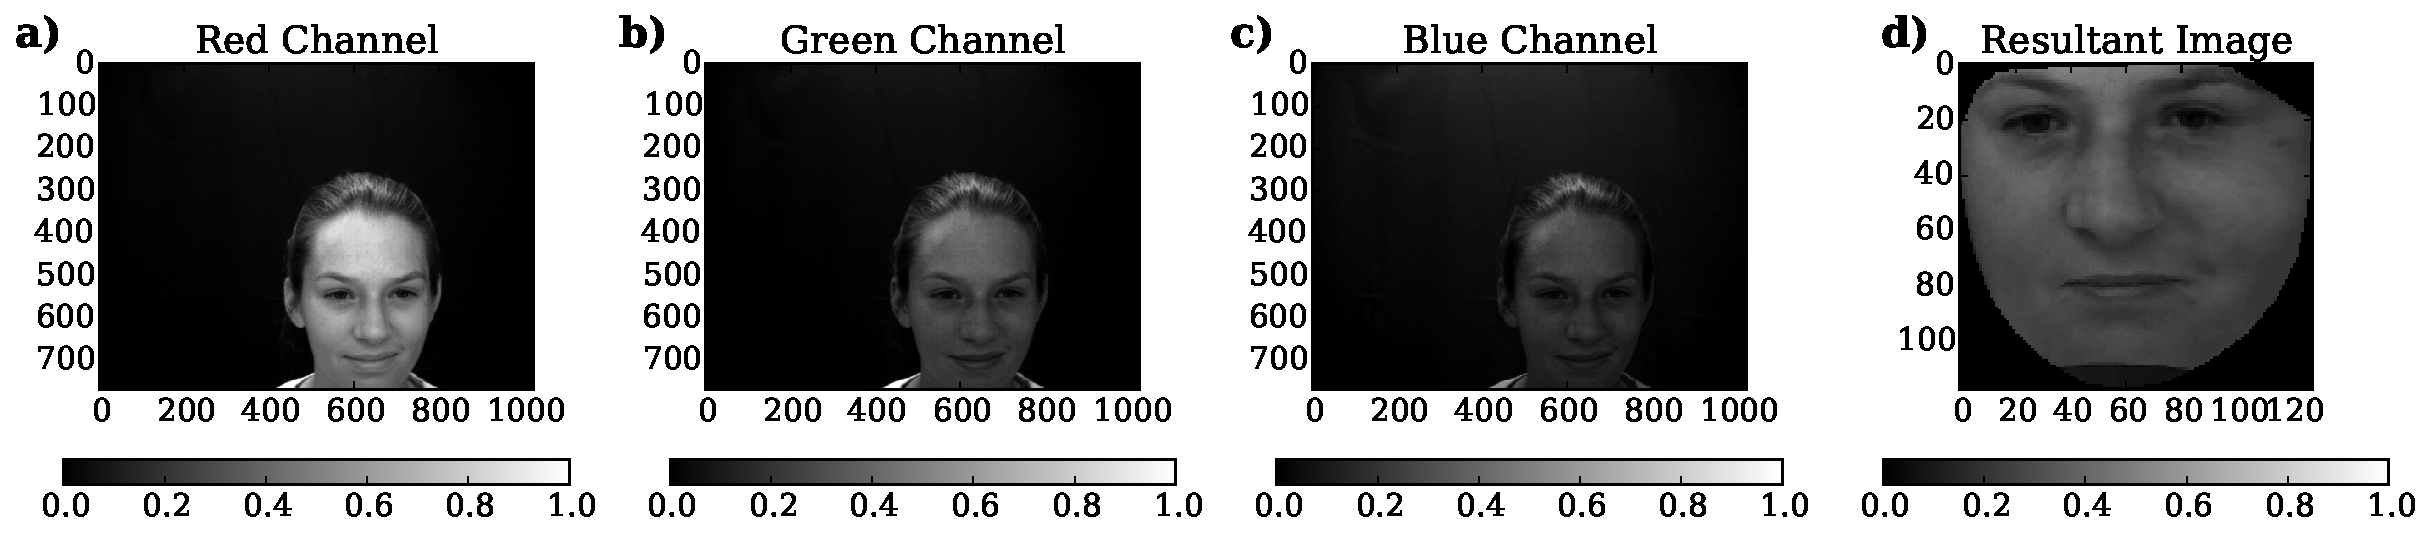
\includegraphics[width =\hsize]{figures/seb_preproc.pdf}
\caption{ {\bf a) b) c)} An example of the original $764 \times 1024$ image with
the 3 RGB channels displayed seperately. {\bf d)} the resultant image
$118 \times 128$ after face registration.} \label{fig:sebproc} \end{figure}

This section defines and visualizes 3 different methods of normalising and scaling
this data which can be combined to create further methods. In order to illustrate
the effect of such operations figures such as figure \ref{fig:faces_none} are used which
show an example face and some statisically generated faces. The ideal method will
have minimum and maximum faces which express high degrees of facial expression, so that
high pixel values can easily be correlated to various AU's in the classifier.

Finally some methods for processing the labels are discussed.

\section{Methods For Images} \label{sec:methods}

\begin{figure}[!h] \centering
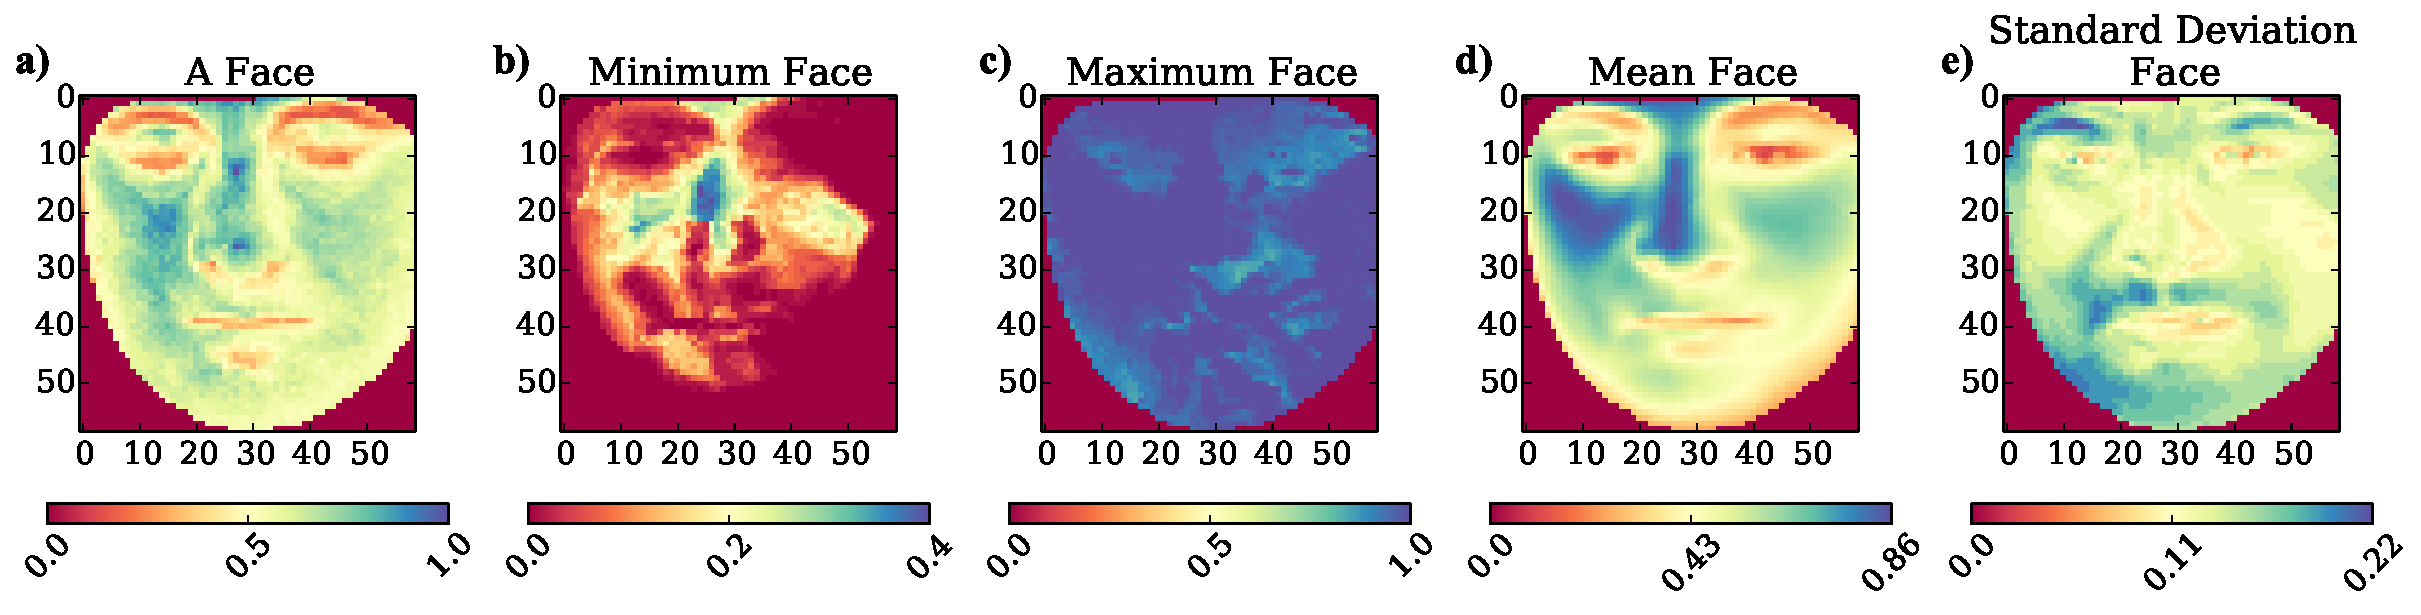
\includegraphics[width =\hsize]{figures/faces.pdf}
\caption{The DISFA dataset with no preprocessing, it shows
the images at the last stage of figure \ref{fig:sebproc}. Plots {\bf b)}, {\bf c)}, {\bf d)}
and {\bf e)}
correspond to the minimum, maximum, mean and standard deviation values of each pixel across
the whole dataset respectively.} \label{fig:faces_none} \end{figure}

The preprocessing methods assume that a dataset of a number of subjects
is described as a matrix of the form:
\begin{equation}
{\bf x} \in \mathbb{R}^{N\times X \times Y},\quad {\bf y} \in \mathbb{N}^{N\times F}
\end{equation}
Where $\mathbf{x}$ contains the images, $\mathbf{y}$ contains the labels,
$N$ is the number of images, $X$ is the width of the image, $Y$ is the height of the
image and $F$ is the number of AU's labeled. Furthermore in some cases an extra dimension
for the subject may be added:
\begin{equation}
{\bf x} \in \mathbb{R}^{S\times N\times X \times Y},\quad {\bf y} \in \mathbb{N}^{S\times N\times F}
\end{equation}
Some subjects may have a slightly different number of frames and this is reflected
in the implementation but not in this section.

Each preprocessing method will be denoted by a function ${\bf P}$ defined as follows:
\begin{equation}
  {\bf P}({\bf x},i) = {\bf x'}_i
\end{equation}
For the per subject case:
\begin{equation}
  {\bf P}({\bf x},i,s) = {\bf x'}_{si}
\end{equation}

This notation aims to express the fact that each image in the resultant dataset
may use information from all other frames. In order to compactly express the operations
we define some statistical operations which clearly show which

\subsection{Contrast Normalisation}
\begin{figure}[!h]
\centering
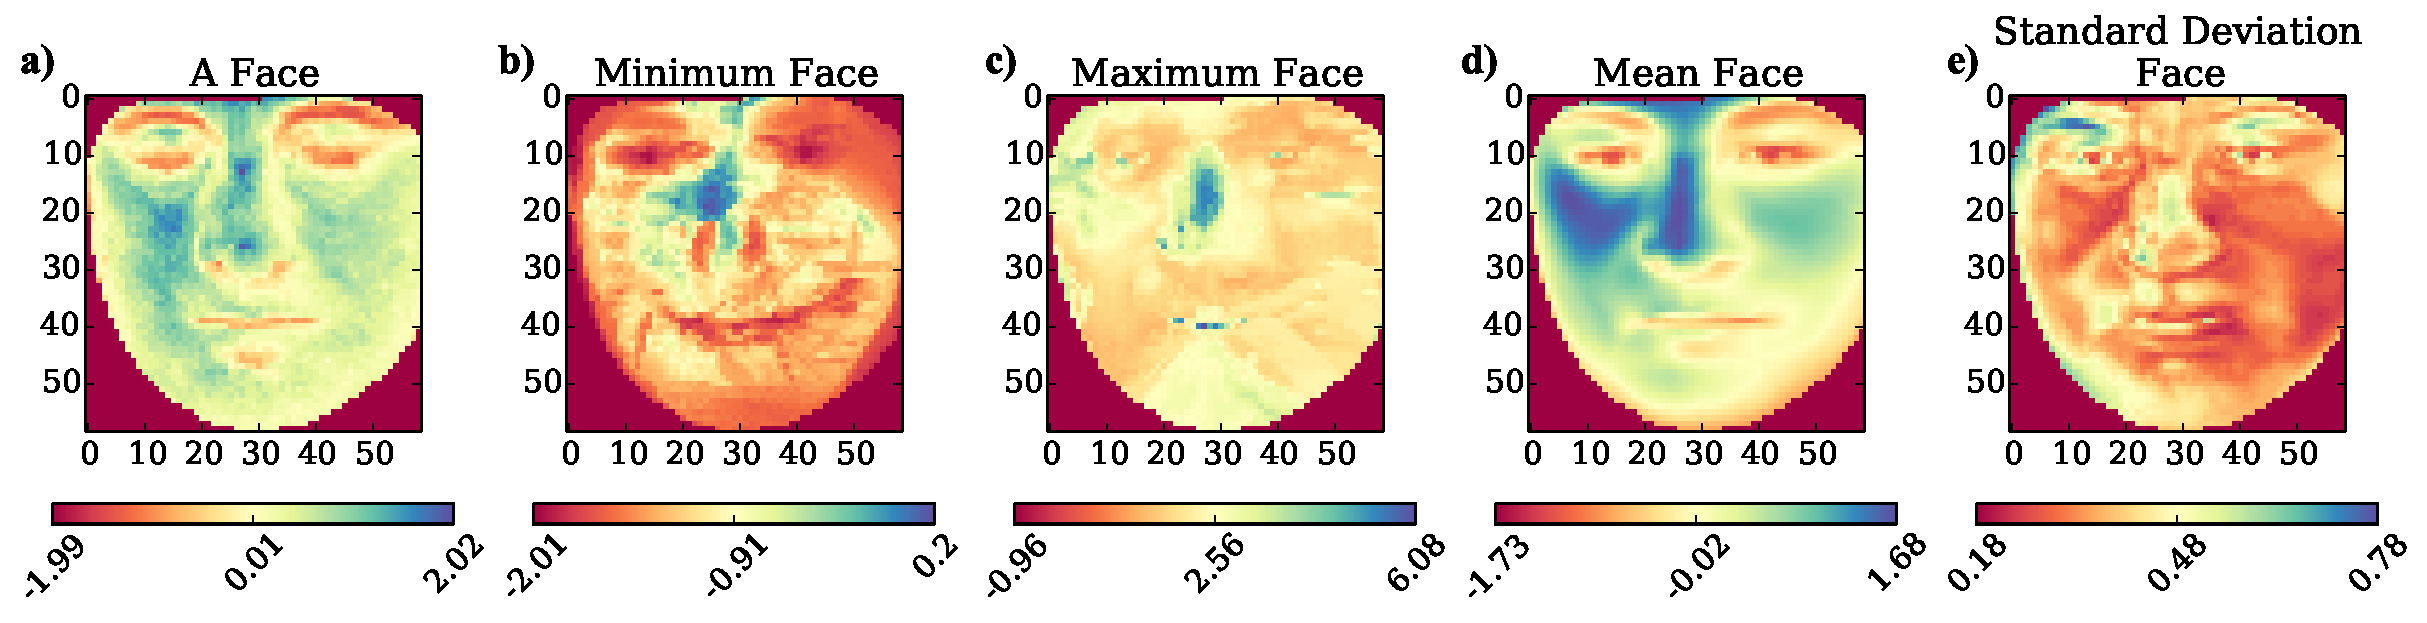
\includegraphics[width =\hsize]{figures/faces_contrast.pdf}
\caption{The DISFA dataset with {\bf contrast normalisation}.
Plots {\bf b)}, {\bf c)}, {\bf d)} and {\bf e)} correspond to the minimum,
maximum, mean and standard deviation values of each pixel across the whole
dataset respectively.}
\label{fig:simple}
\end{figure}

For each image find the mean pixel value and standard deviation and then subtract the mean
and divide by the standard deviation. This standardises the amount of contrast in each image.
\begin{equation}
   P({\bf x},i)= ({\bf x}_{ijk} - \mu({\bf x}_{i}))/\sigma ({\bf x}_{i}) = {\bf x}_{ijk}'
   \label{eq:con}
\end{equation}
Where $\mu$ and $\sigma$ gives the mean and standard deviation value of a matrix respectively.
Equation \ref{eq:con} shows this, a disadvantage of this normalisation is that it
has no regard of facial structures.
\subsection{Mean Face Normalisation}
Here the mean face and standard deviation face is subtracted and divided away from the
image, these faces might be per subject or per dataset, as shown:
\begin{equation}
  P({\bf x},i) =  ({\bf x}_{i} - {\boldsymbol \mu}_0( {\bf x}))/{\boldsymbol \sigma}_0({\bf x}_{i})  = {\bf x}_{i}'
\end{equation}
\begin{equation}
  P_s({\bf x},s,i) = ({\bf x}_{si} - {\boldsymbol \mu}_{0,1}( {\bf x}_s))/{\boldsymbol \sigma}_{0,1}( {\bf x}_s))  = {\bf x}_{si}'
\end{equation}
Where ${\boldsymbol \mu}_{i,j..}$ denotes the mean over the axes $i,j..$ and
similarly for ${\boldsymbol \sigma} $ the standard deviation.
The point of this normalisaiton is to enhance the intensity of any pixels which
are unusal, these pixels should hold most information about potential facial expressions.
\begin{figure}[!h] \centering
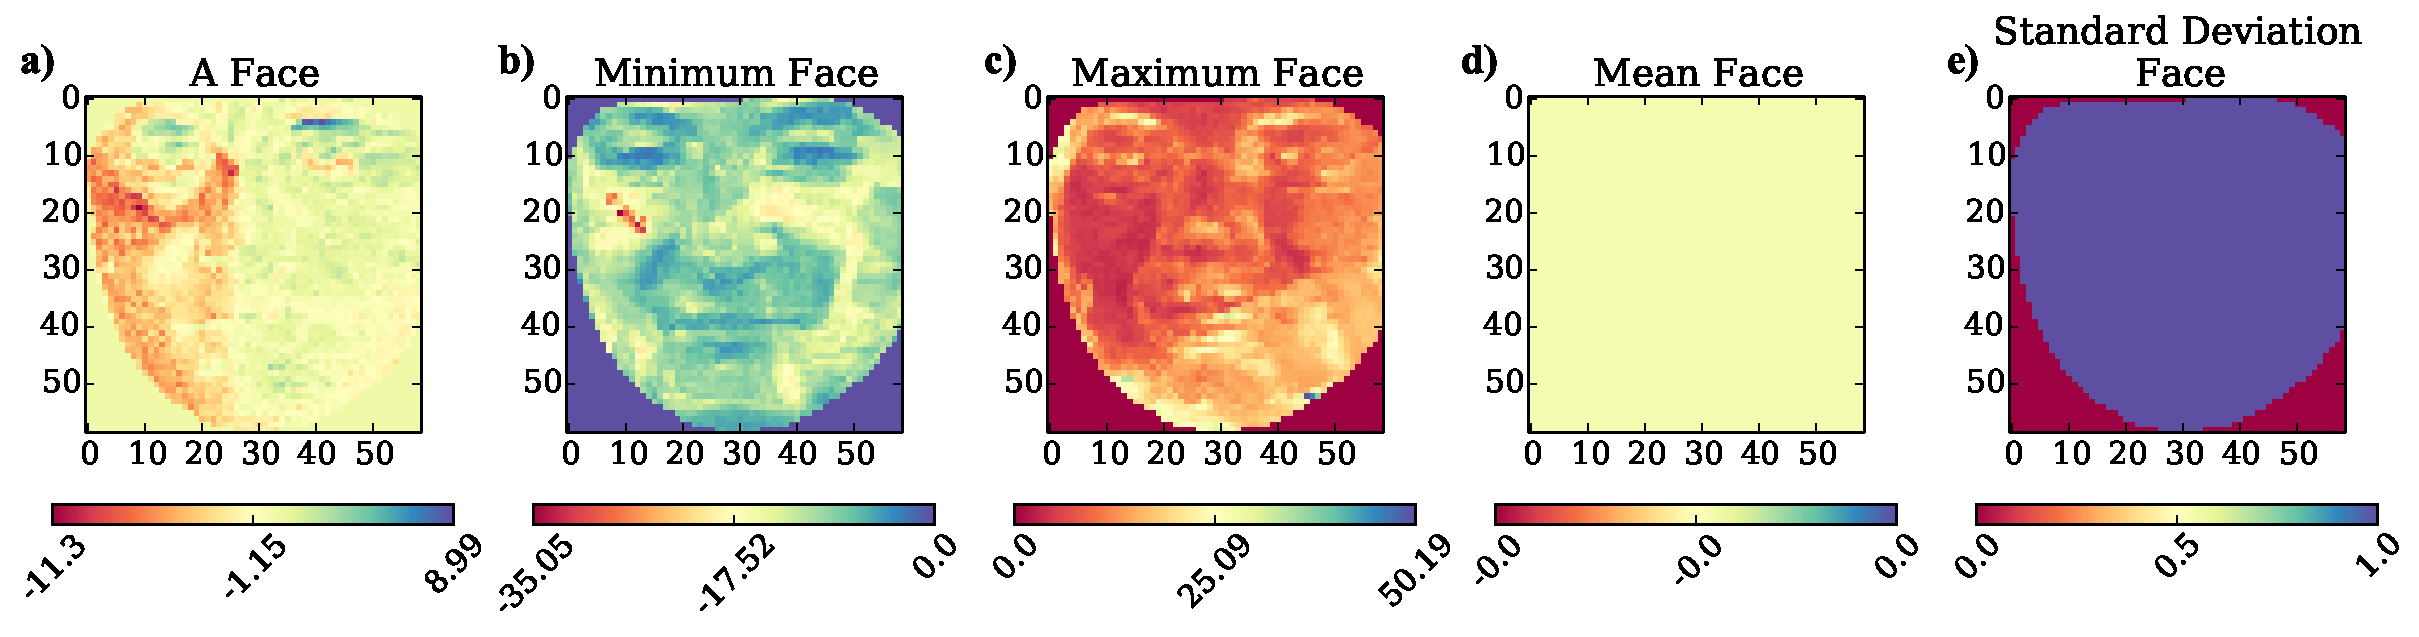
\includegraphics[width =\hsize]{figures/faces_per_subject_face.pdf}
\caption{The DISFA dataset with {\bf per subject mean face normalisation}.
Plots {\bf b)}, {\bf c)}, {\bf d)} and {\bf e)} correspond to the minimum,
maximum, mean and standard deviation values of each pixel across the whole
dataset respectively.}
\label{fig:}
\end{figure}
\subsection{Range Scaling}
This normalisation stretches the data between -1 and 1, this contains no feature engineering
intution but is simply another type of normalisation to try.
\begin{equation}
  {\boldsymbol r}({\bf x})_{axis} = {\boldsymbol \min}_{axis}({\bf x}) - {\boldsymbol \min}_{axis}({\bf x})
\end{equation}
\begin{equation}
   P({\bf x},i) =
   \frac{{\bf x}_{i} - \frac{1}{2}\left ( {\boldsymbol \min}_0({\bf x}) + {\boldsymbol \min}_0({\bf x}) \right ) }{\frac{1}{2}{\boldsymbol r}_0({\bf x})}
   = {\bf x}_{i}'
\end{equation}
For the per subject case:
\begin{equation}
   P_s({\bf x},i,s) =
   \frac{{\bf x}_{si} - {\boldsymbol \min}_0({\bf x}_s) - \frac{1}{2}{\boldsymbol r}_0({\bf x}_s) }{\frac{1}{2}{\boldsymbol r}_0({\bf x}_s)}
   = {\bf x}_{si}'
\end{equation}
\begin{figure}[!h] \centering
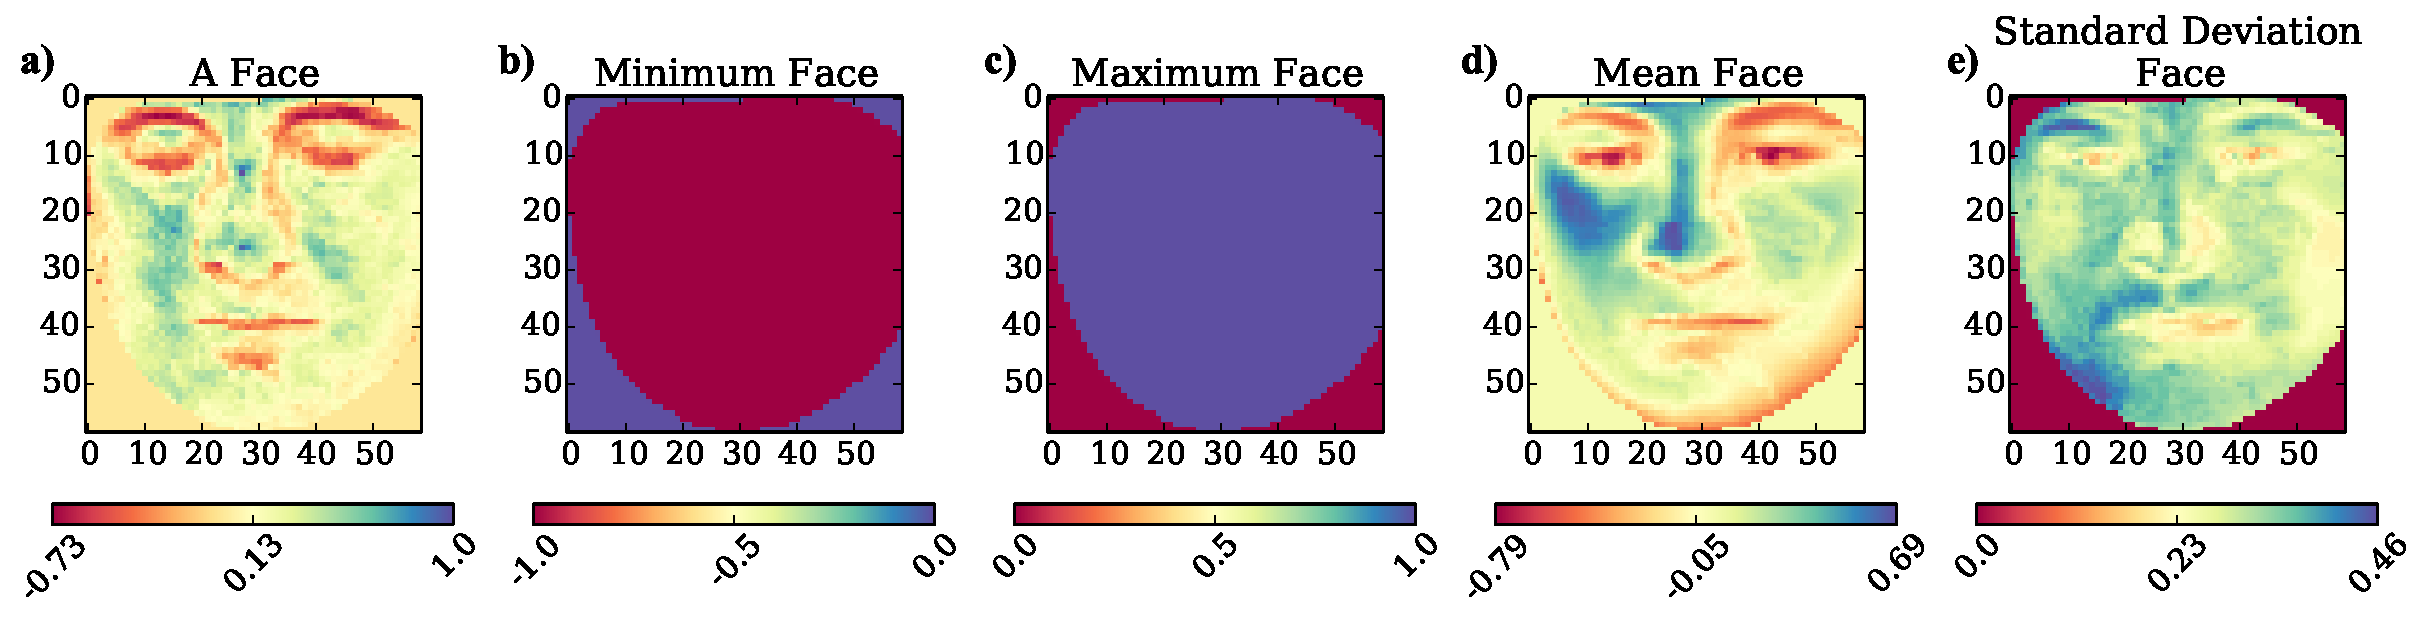
\includegraphics[width =\hsize]{figures/faces_range.pdf}
\caption{The DISFA dataset with {\bf range scaling between -1 and 1}.
Plots {\bf b)}, {\bf c)}, {\bf d)} and {\bf e)} correspond to the minimum,
maximum, mean and standard deviation values of each pixel across the whole
dataset respectively.} \label{fig:simple} \end{figure}
\subsection{Combining methods}
Some methods can be combined, figures \ref{fig:faces_contrast_face} and \ref{fig:faces_per_subject_contrast_face}
shows the result of combining the mean face subtraction and then the
contrast normalisation (in the per subject and whole set cases respectively). It is clear the effect is to
reduce the range of the data, which may be useful for the classifier, however parts of the image
which were all zero are now not which may result in lower performance.

\begin{figure}[!h] \centering
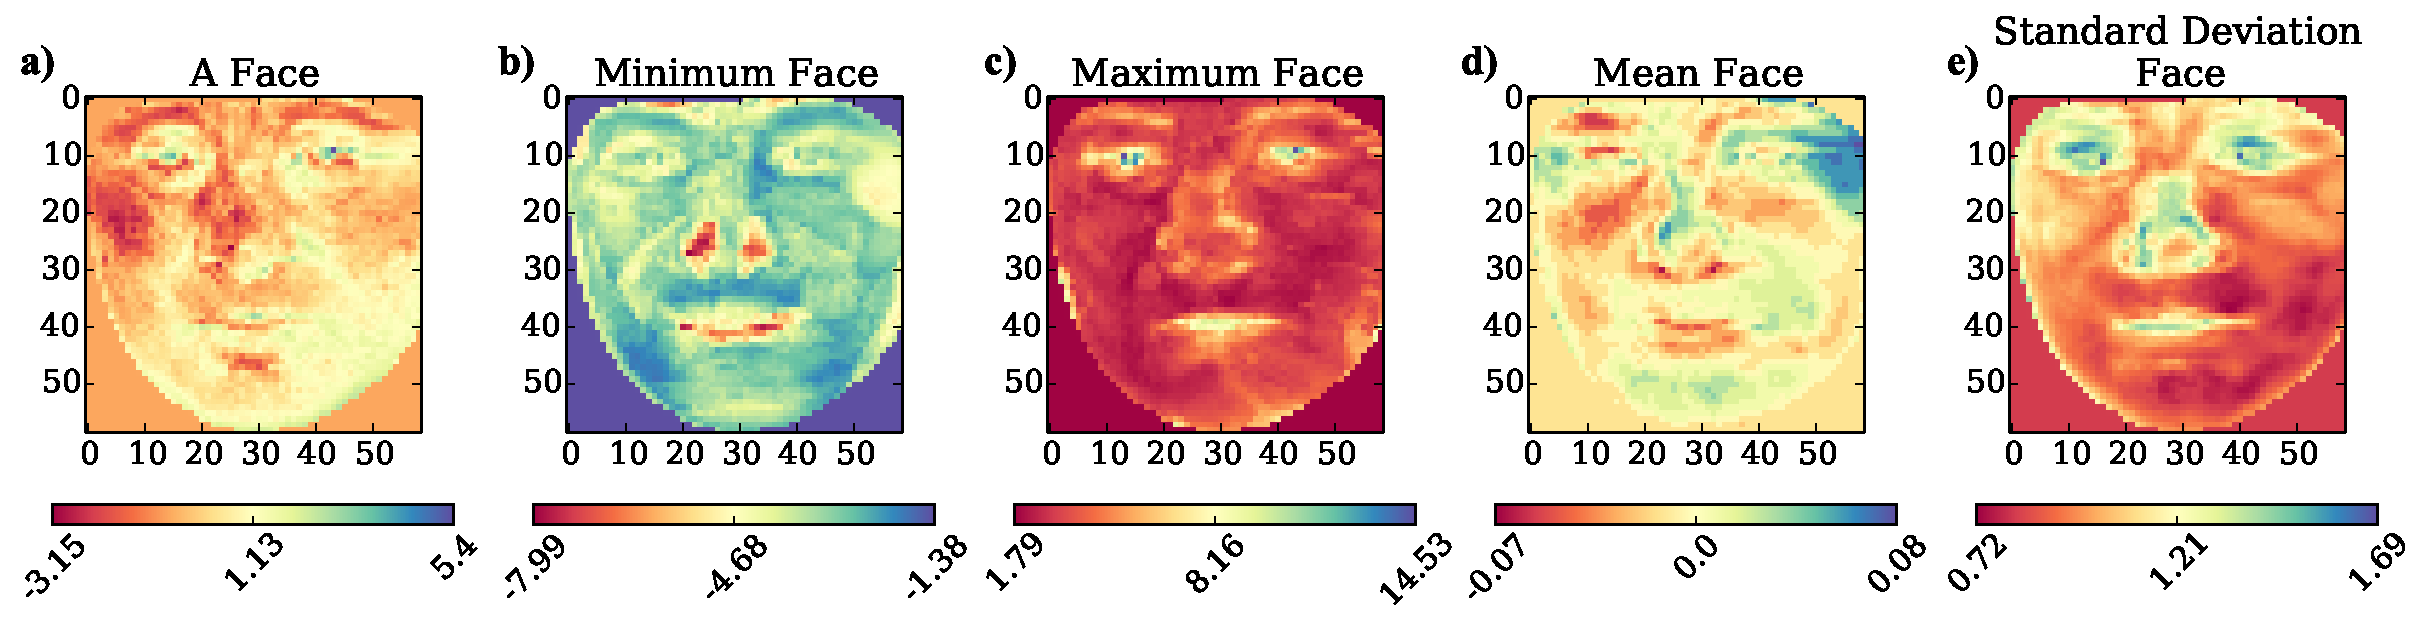
\includegraphics[width =\hsize]{figures/faces_contrast_face.pdf}
\caption{The DISFA dataset with {\bf mean face normalisation and then contrast normalisation} applied.
Plots {\bf b)}, {\bf c)}, {\bf d)} and {\bf e)} correspond to the minimum,
maximum, mean and standard deviation values of each pixel across the whole
dataset respectively.} \label{fig:faces_contrast_face} \end{figure}

\begin{figure}[!h] \centering
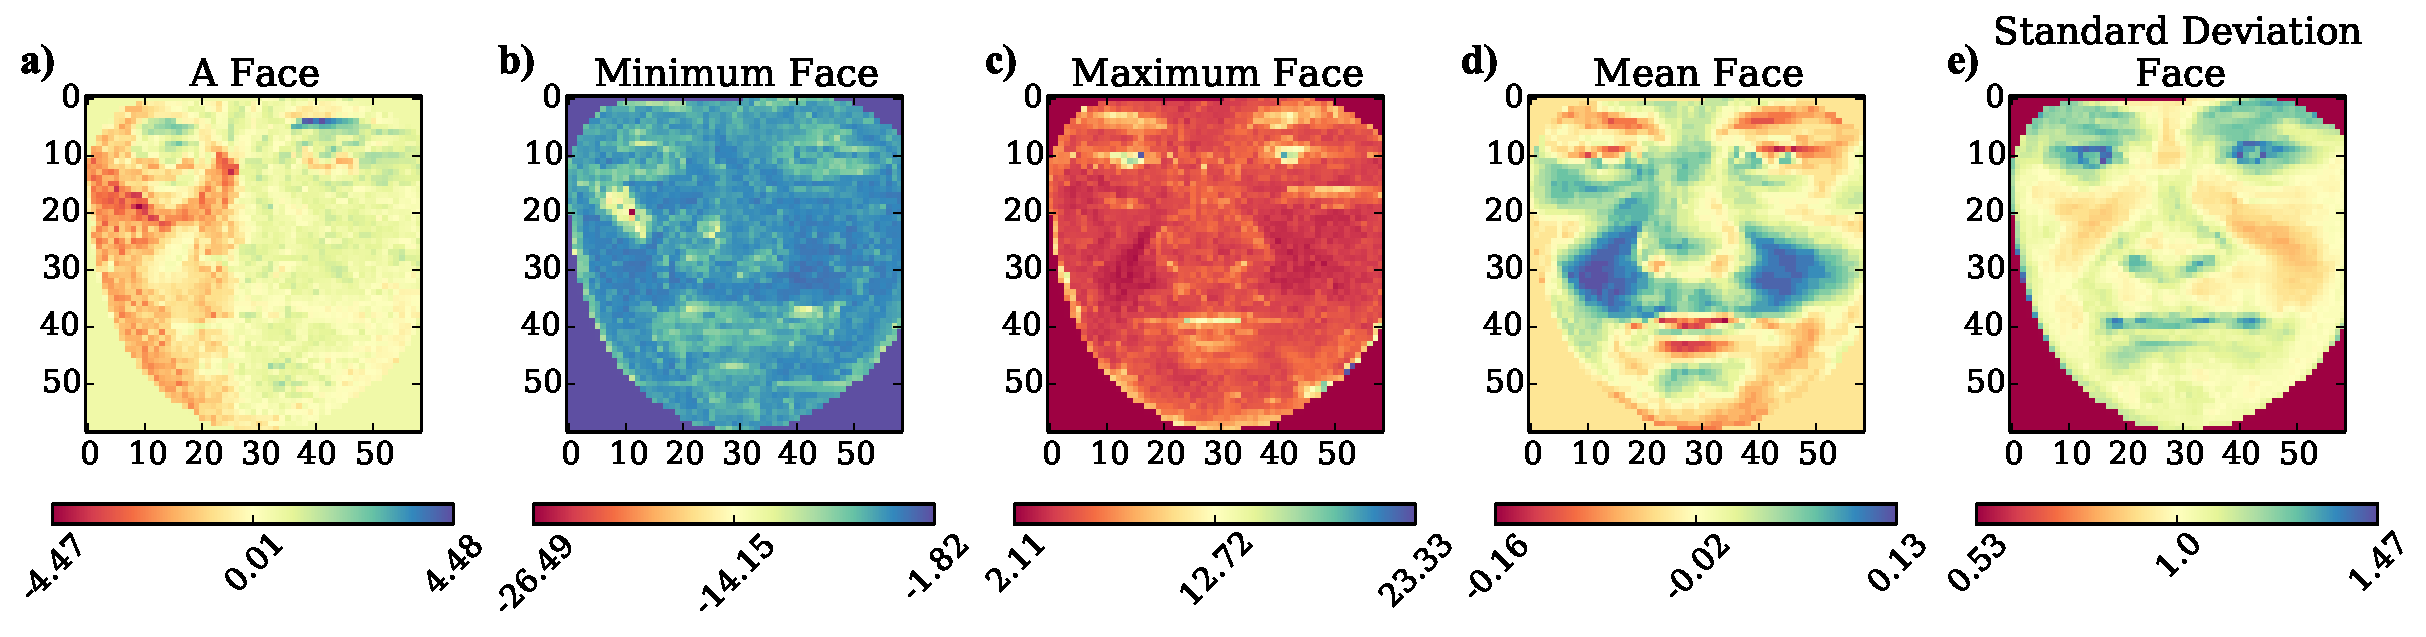
\includegraphics[width =\hsize]{figures/faces_per_subject_contrast_face.pdf}
\caption{The DISFA dataset with {\bf per subject mean face normalisation and then contrast normalisation} applied.
Plots {\bf b)}, {\bf c)}, {\bf d)} and {\bf e)} correspond to the minimum,
maximum, mean and standard deviation values of each pixel across the whole
dataset respectively.} \label{fig:faces_per_subject_contrast_face} \end{figure}

\subsection{Masking}
From figure \ref{fig:faces_none} it is evident some pixels have a maximum and minimum value
of zero and no deviation. This means there is no information in these areas and hence
the would ideally not even know about them. If the network was a set of fully connected layers
these pixels could just be removed from the system, however convolutional layers require
rectangular inputs and so a solution is to apply a mask at the level of the cost function.

As this applies only to the autoencoder who has a cost function (equation \ref{eq:autoencoder_cost}):
\begin{equation}
    J(\tilde{\mathbf{x}},\tilde{\mathbf{y}})
    = \frac{1}{N}\left |\mathbf{y}(\tilde{\mathbf{x}})-\tilde{\mathbf{x}}\right | ^2
\end{equation}
Instead becomes:
\begin{equation}
    J(\tilde{\mathbf{x}},\tilde{\mathbf{y}})
    = \frac{1}{N}\left |\mathbf{y}(\tilde{\mathbf{x}}) \odot \mathbf{M}-\tilde{\mathbf{x}}\right | ^2
\end{equation}

Where M is a two dimensional matrix with elements unity where the dataset is nonzero
and zero when the dataset is zero for that pixel. Here $\odot$ denotes an elementwise
product between two matrices.

\section{Methods For Labels}

As breifly discussed earlier in this section, the labels are defined as a matrix:
\begin{equation}
  {\bf y} \in \{0,1,2,3,4,5\}^{N\times F}
\end{equation}

Where 5 is the highest intensity for an AU and 0 is the abscence of that AU.
Typically a neural network outputs values between 0 and 1 so these values are divided by 5 to make them compatible.
For an intensity estimation problem that is all that is required, however for classification
the AU labels need to binary and so a threshold is chosen at which an AU is considered present.
Finally in some cases such as the one described in section \ref{sec:binsoft} the label vector
needs to be expanded to also contain the negative case for presence, hence doubling its size.

\subsection{Train, Test and Validation set split}

Splitting the data is important, this is how it was done.
\subsubsection{Splitting Method 1} \label{sec:splitting}
\begin{table}[h!]
  \centering
  \begin{tabular}{|l|l|}
  \hline
  set & subjects   \\
  \hline
   Train          & 2,4,6,8,10,12,16,18,23,25,27,29,31      \\
  \hline
  Validation      & 1,3,5,7,9,11,13,17,21,24,26,28,30,32 minus test set     \\
  \hline
  Test           & 500 chosen randomly taken from validation set      \\
 \hline
  \end{tabular}
  \caption{Typical split of the DISFA dataset for experimentation perposes}
  \label{sec:splitting}
\end{table}

\chapter{Modelling DISFA} \label{sec:model}
  This chapter describes the path taken in constructing the autoencoding classifier (AEC) network, detailing
  the experiments which were performed to create the final configuration.
  The most important metric used to judge a network in the chapter is the Average ROC score of the classifier
  when applied to the un-seen validation set\footnote{}, the secondary metric will be the error
  in the reconstructed image outputted from the autoencoder. The overall aim is to
  find a configuration where improving the secondary metric (the autoencoder) improves
  the primary metric (the classifier) and that the presence of the autoencoder improves
  the performance of the classifier.

  \begin{figure}[h!]
   \centering
   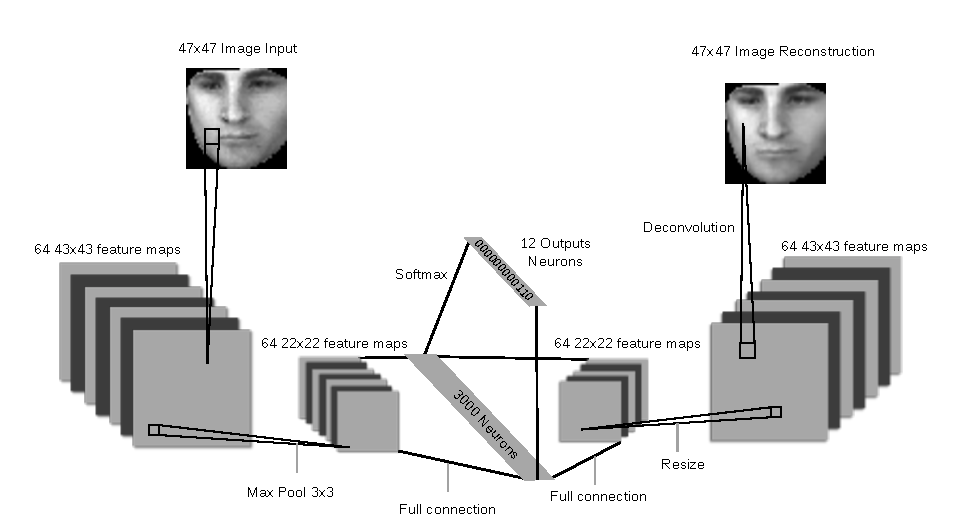
\includegraphics[width=\textwidth]{illustrations/aec_network.pdf}
   \captionof{figure}{General structure of the proposed network. Each rectangle
   represents many layers of neurons and the thin lines represent connections between layers.}
  \end{figure}

  The results will show, that it is unclear if there is a direct relationship, nonetheless
  the work is a detailed exploration of how autoencoders and classifiers interact with each other
  under various preprocessing situations and different autoencoder transfer functions \footnote{These describe the degree to which
  each cost function is trained during training, section \ref{sec:autoalpha} details this in full.}.

  \section{Experimental set up}
    In order to develop the network for modelling the DISFA dataset a set of common
    parameters for experimentation are useful to define, these are shown in table \ref{tab:common}

    \begin{table}[!h]
      \centering { \footnotesize
      \begin{tabular}{ll}
        \hline
        \textbf{Parameter}                       & \textbf{Value}                \\ \hline
        Optimizer                                & Adam                          \\
        Learning Rate                            & 0.001                         \\
        L2 Regularisation Coefficient            & 0.0                           \\
        Hidden layer activation functions         & ReLu                          \\
        Image downscaling                        & 0.4                           \\
        AU's present                             & 1,2,4,5,6,9,12,15,17,20,25,26 \\
        Iterations:                              & 1000                          \\
        Early model save percent                 & 50\%                          \\
        Weight tensor initial standard deviation & 0.001                         \\
        Bias tensor initial value                & 0.01                          \\
        Validation batch size                    & 500                           \\
        Penultimate fully connected layer size   & 3000                          \\
        \hline
      \end{tabular}
      \caption{Common parameters for most experiments in the section. These parameters should be
      assumed in proceeding sections unless otherwise stated.} \label{tab:common} }
    \end{table}


  % A single hidden layer
  % A single hidden layer
  % A single hidden layer
  % A single hidden layer
  \section{A single hidden layer}
    \begin{table}[h!]
    \centering
    {\footnotesize
    \begin{tabular}{|lllllllll|}
    \hline
    \multicolumn{1}{|l|}{Element} & Type     & \multicolumn{1}{l|}{Dimensions}                     & Type     & \multicolumn{1}{l|}{Dimensions}                      \\ \hline
    \multicolumn{1}{|l|}{x}       &          & \multicolumn{1}{l|}{$47\times47\times1$}            &          & \multicolumn{1}{l|}{}                                \\ \hline
    \multicolumn{1}{|l|}{$L_1$}   & fc       & \multicolumn{1}{l|}{$2209\times14$}              & Binary Softmax & \multicolumn{1}{l|}{$3000\times2\times12$}        \\
    \multicolumn{1}{|l|}{$y_1$}   & dropout  & \multicolumn{1}{l|}{$14$}                         &          & \multicolumn{1}{l|}{$24$}                              \\ \hline
    \multicolumn{1}{|l|}{$L_2$}   & fc       & \multicolumn{1}{l|}{$14\times2209$}              &          & \multicolumn{1}{l|}{}                                   \\
    \multicolumn{1}{|l|}{$y_2$}   &          & \multicolumn{1}{l|}{$3000$}                         &          & \multicolumn{1}{l|}{}                                \\ \hline
    \multicolumn{1}{|l|}{$L_3$}   & reshape & \multicolumn{1}{l|}{}                    &          & \multicolumn{1}{l|}{}                                \\
    \multicolumn{1}{|l|}{$y_3$}   &          & \multicolumn{1}{l|}{$47\times47\times 1$}          &          & \multicolumn{1}{l|}{}                                \\ \hline
    \end{tabular}

    \caption{} \label{net:simple1}

    }
    \end{table}
    %ID = 4 date = '2016_08_14' group = 'alpha'
    As an introduction to the types of results that will be used to evaluate various
    models, this section shows the performance of a neural network with one
    hidden layer. This also should provide a worst case for classification and autoencoding performance.

    The structure of this network is shown in table \ref{net:simple1}, 14 neurons
    are chosen heuristically as there are 14 AU's and one might naively hope that the number of
    neurons required in the hidden layer would be equal to the number of features. Per subject face normalisation
    is chosen from section \ref{sec:meanface} and the images are scaled to be size $118 \times 118$.
    Figure \ref{fig:simple} shows the losses during training, on the train and validation set where table \ref{tab:splitting}
    describes the way the data is partitioned. Over fitting to the train set is evident very early in the training, there are two
    possible reasons, firstly the validation set might be too small to represent all AU's and secondly the model is still quite basic.
    Training the classifier reduces the performance of the autoencoder visibly.

    \begin{table}[h!]
      \centering
      {\footnotesize
      \begin{tabular}{|l|l|}
      \hline
      set & subjects   \\
      \hline
       Train          & 2,4,6,8,10,12,16,18,23,25,27,29,31      \\
      \hline
      Test      & 1,3,5,7,9,11,13,17,21,24,26,28,30,32 minus validation set     \\
      \hline
      Validation           & 500 chosen randomly taken from test set      \\
     \hline
      \end{tabular}
      \caption{Typical split of the DISFA dataset for experimentation purposes}
      \label{tab:splitting}  }
    \end{table}


    \begin{figure}[!h]
    \centering
    \includegraphics[width =\hsize]{../graphs/losses_2016_08_14_004.pdf}
    \caption{The losses of a neural network consisting of a $118^2$ neuron input layer, a 14
    neuron hidden layer, a branch of the same size as the input layer for autoencoding
    and branches for binary softmax classifiers for each AU. The classifier mean
    squared loss is shown only for interest, the network trains by minimising
    the cross entropy. The $\alpha$ coefficient determines the balance between the
    classifier and the autoencoder losses, $\alpha=1$ signifies only autoencoder training
    while $\alpha=0$ means only classifier training. Over fitting is observed
    on all loss functions. Training the classifier
    overwrites the weights and hence ends up reducing
    the performance of the autoencoder.}
    \label{fig:simple}
    \end{figure}

    \begin{table}[!h]
    \centering
    {\small
    \begin{tabular}{llllll}
    \hline
    \textbf{Class}    & \textbf{ROC} & \textbf{ROC} & \textbf{Max F1} & \textbf{Max Precision} & \textbf{Max Recall} \\ \hline
    1                 & 0.5          & fail         & 0.09            & 0.06                   & 1.0                 \\
    2                 & 0.6          & poor         & 0.07            & 0.05                   & 1.0                 \\
    4                 & 0.62         & poor         & 0.31            & 0.27                   & 1.0                 \\
    5                 & 0.49         & fail         & 0.02            & 0.02                   & 1.0                 \\
    6                 & 0.8          & fair         & 0.48            & 0.42                   & 1.0                 \\
    9                 & 0.46         & fail         & 0.11            & 0.06                   & 1.0                 \\
    12                & 0.89         & good         & 0.67            & 0.73                   & 1.0                 \\
    15                & 0.46         & fail         & 0.11            & 0.06                   & 1.0                 \\
    17                & 0.55         & fail         & 0.18            & 0.25                   & 1.0                 \\
    20                & 0.51         & fail         & 0.09            & 0.12                   & 1.0                 \\
    25                & 0.65         & poor         & 0.51            & 0.42                   & 1.0                 \\
    26                & 0.57         & fail         & 0.32            & 0.23                   & 1.0                 \\ \hline
    \textbf{Average:} & 0.59         & fail         & 0.25            & 0.22                   & 1.0                 \\ \hline
    \end{tabular} }
    \caption{}
    \label{my-label}
    \end{table}


    \newpage
    %
    %
    %
    %
  \section{Joint classification}

    Typical deep neural networks are used to classify
    one image into only one category. The case with the DISFA dataset is different, we
    would like to be able to classify the categories jointly,  putting one frame into more than
    one AU category. Ideally the network would output a confidence score between 0 and 1
    to signify if an AU is present and we would calculate some optimum threshold value
    (ideally this would be 0.5).

    The following list details three possible solutions to the joint classification problem:

    \begin{itemize} \label{sec:binsoft}
      \item {\bf Softmax Layer} - This is a traditional, fully connected layer with
                                  a softmax activation function (see equation \ref{eq:softmax}).
                                  The issue with this is that it provides a probability distribution over AUs
                                  but the required quantity is a probability distribution for each AU. In the implementation
                                  the negative neuron of each binary layer is only used for training purposes, and it is
                                  discarded while evaluating the classification performance.
      \item {\bf Sigmoid Layer} - This again is like the previous solution but instead each neuron gives a confidence
                                  score between 0 and 1 for each AU with a sigmoid function (see equation \ref{eq:sigmoid}).
                                  The issue with this however is that sigmoid
                                  functions have vanishing gradients at large input values
                                  hence training may become difficult.
      \item {\bf Binary Softmax Layers} - Here there is a two neuron softmax layer
                                          for each AU, this doubles the amount of weights
                                          but gives a probability over the presence and
                                          absence of each AU which is ideal.
    \end{itemize}

    Table \ref{net:classcompnet} compares how each of these solutions perform using the network described in
    tables \ref{net:classcompnet}, this network was chosen because it contains all of the main
    components of larger networks typically used for classification tasks, such as a convolutional
    layer, max pool layer and fully connected layer. It contains the autoencoder section which will be
    explored later on in the section mainly out of interest.

    \begin{table}[h!]
    \centering
    {\footnotesize
    \begin{tabular}{|lllllllll|}
    \hline
    \multicolumn{1}{|l|}{Element} & Type     & \multicolumn{1}{l|}{Dimensions}                     & Type     & \multicolumn{1}{l|}{Dimensions} \\ \hline
    \multicolumn{1}{|l|}{x}       &          & \multicolumn{1}{l|}{$47\times47\times1$}            &          & \multicolumn{1}{l|}{}          \\ \hline
    \multicolumn{1}{|l|}{$L_1$}   & conv 1   & \multicolumn{1}{l|}{$5\times 5\times1\times 64$}    &          & \multicolumn{1}{l|}{}          \\
    \multicolumn{1}{|l|}{$y_1$}   &          & \multicolumn{1}{l|}{$43\times43\times64$}           &          & \multicolumn{1}{l|}{}          \\ \hline
    \multicolumn{1}{|l|}{$L_2$}   & max pool & \multicolumn{1}{l|}{$2\times 2$}                    &          & \multicolumn{1}{l|}{}          \\
    \multicolumn{1}{|l|}{$y_2$}   &          & \multicolumn{1}{l|}{$22\times22\times 64$}          &          & \multicolumn{1}{l|}{}          \\ \hline
    \multicolumn{1}{|l|}{$L_3$}   & fc       & \multicolumn{1}{l|}{$30976\times3000$}              & \multicolumn{2}{l|}{Sotmax Layer or}      \\
    \multicolumn{1}{|l|}{$y_3$}   &          & \multicolumn{1}{l|}{}                               & \multicolumn{2}{l|}{Sigmoid Layer or}     \\
    \multicolumn{1}{|l|}{$L_4$}   & dropout  & \multicolumn{1}{l|}{$3000$}                         & \multicolumn{2}{l|}{Binary Softmax Layer} \\
    \multicolumn{1}{|l|}{$y_4$}   &          & \multicolumn{1}{l|}{}                               &          & \multicolumn{1}{l|}{}          \\ \hline
    \multicolumn{1}{|l|}{$L_5$}   & resize\& reshape & \multicolumn{1}{l|}{$2$}                    &          & \multicolumn{1}{l|}{}          \\
    \multicolumn{1}{|l|}{$y_5$}   &          & \multicolumn{1}{l|}{$43\times43\times 64$}          &          & \multicolumn{1}{l|}{}          \\ \hline
    \multicolumn{1}{|l|}{$L_6$}   & deconv 1   & \multicolumn{1}{l|}{$5\times 5\times1\times 64$}  &          & \multicolumn{1}{l|}{}\\
    \multicolumn{1}{|l|}{$y_6$}   &          & \multicolumn{1}{l|}{$47\times47\times1$}            &          & \multicolumn{1}{l|}{}         \\ \hline
    \end{tabular}

    \caption{Set up for deciding on which final layer structure to use.
    This network is very similar to \textbf{Network 1} which is described later in the section.} \label{net:classcompnet}

    }
    \end{table}


    \begin{table}[!h] {\footnotesize
      \centering
      \begin{tabular}{lccc}
      \hline
      Final Layer   & Av. ROC &   Av. Best F1 &   Autoencoder Loss (Not normalised) \\
      \hline
      Binary Softmax Layers  &   0.73 &  0.34 &   20.7 \\
      Softmax Layer          &   0.69 &  0.30 &   15.8 \\
      Sigmoid Layer          &   0.50 &  0.19 &  126.2 \\
      \hline
      \end{tabular}
    \caption{Comparison of the three ways the final layer could be implemented using network 1 (see table \ref{compnet})} \label{net:classcompnet} }
    \end{table}

    The results show that the binary softmax layer outperforms the other solutions. The
    softmax layer is only slightly worse, but in order to accommodate for the potential of higher rates
    it is clear that the binary softmax is the better choice. This is because, in joint classification problems
    the simple softmax layer struggles to report more than 2 AU's as the outputs must add up to one.
    The low performance of the softmax layer is interesting and one reason might be that of vanishing gradients due to
    the bottleneck layer containing high activation values.

    As the softmax layer is better in the results and has a better potential for good results
    it is chosen as the classifier for the rest of this work.

  %
  %
  %
  %
  \section{Autoencoder classifier balancing} \label{sec:autoalpha}
    A key structure that is to be investigated in this report is a network with two objective functions:
    autoencoder and classifier. This is achieved by having a bottleneck layer where the branching occurs.
    The autoencoder has symmetry along this bottleneck, while the classifier consists of one further layer
    (the binary softmax classifier from the previous section). The cost function for the whole network is as follows:

    \begin{equation}
        J(\tilde{\mathbf{x}},\tilde{\mathbf{y}}) = -\frac{1-\alpha(t)}{2FN}\tilde{\mathbf{y}}\cdot\log(\mathbf{y}(\tilde{\mathbf{x}}))
        + \frac{\alpha(t)}{N}\left |\mathbf{y}(\tilde{\mathbf{x}}) \odot \mathbf{M}-\tilde{\mathbf{x}}\right | ^2
    \end{equation}

    Here F is the number of AU's, N is the size of the batch and $\alpha(t)$ is a
    function which balances the two costs. $\alpha(t)$ might be constant $\left ( \alpha_{\text{constant}}(t)=\frac{1}{2} \right )$ or
    some sort of polynomial which stays in the range $[0,1]$.

    For much of the initial investigations we employ:
    \begin{equation}
    \alpha_{\text{step}}(t,p,T) =
    \begin{cases}
      1           & \text{if}\ t<pT \\
      0           & \text{otherwise}
    \end{cases}
    \end{equation}

    Where t indexes iterations, T is the total number of iterations and p is the
    percentage of iterations that should be in the first region of the piecewise function
    where $\alpha=1$.
    This nicely expresses what is typically meant by pre-training in the literature, it trains
    the autoencoder up until iteration $pT$ (normally $p=\frac{1}{2}$ or $p=\frac{2}{3}$) and then the classifier for the remainder of the time.
    This acts as a good base case to test both sides of the network, later more interesting
    functions will be explored such as the sigmoid step:

    \begin{equation}
      \alpha_{\text{sigmoid}}(t,T,p,\tau) = \frac{1}{1 + \exp(1 + \tau (t/T - p))}
    \end{equation}

    Or a polynomial function:

    \begin{equation}
      \alpha_{\text{poly}}(t,T,n) = 1 - \left ( \frac{t}{T} \right )^n
    \end{equation}

    Or a periodic step function:

    \begin{equation}
    \alpha_{\text{alternate}}(t,p,T) =
    \begin{cases}
      1           & \text{if } t < |T/p| \text{ and } p > 0\\
      0           & \text{if } t < |T/p| \text{ and } p \leq 0\\
      \alpha_{\text{alternate}}(t-|T/p|,-p,T)           & \text{otherwise} \\
    \end{cases}
    \end{equation}

    Examples of such functions are plotted in figure \ref{fig:alpha_functions}.

    \begin{figure}[!h]
    \centering
    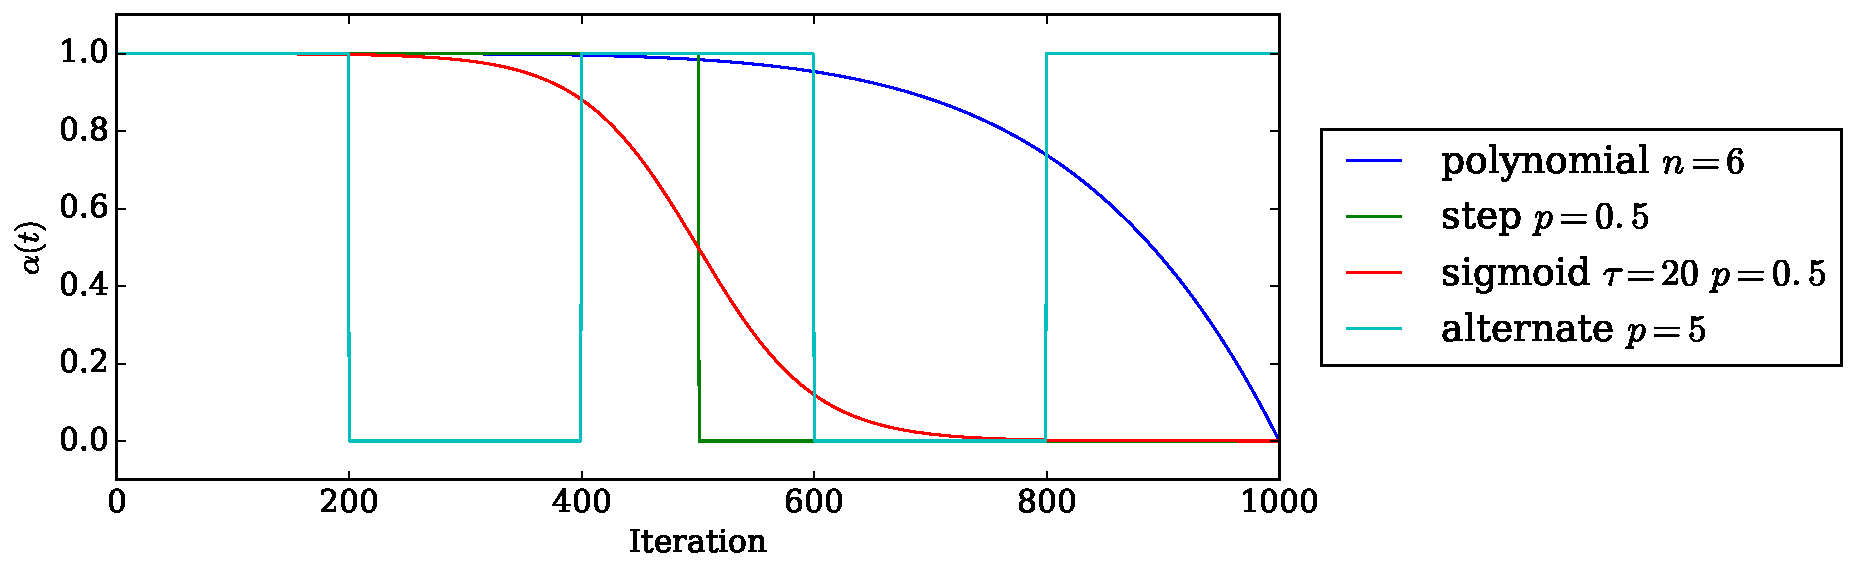
\includegraphics[width =\hsize]{figures/alpha.pdf}
    \caption{Examples of alpha functions described in section \ref{sec:autoalpha}
    for the polynomial case higher values of $n$ decrease the amount of training
    the classifier receives. While in the case of the step p dictates the training
    that each network receives, the sigmoid can be seen as a smoothed out step function
    with the two being equivalent as $ \tau \rightarrow \infty$. Similarly as $n \rightarrow \infty$
    the polynomial function turns into a constant function with $c=1$ except at the final
    iteration.}
    \label{fig:alpha_functions}
    \end{figure}

    % def alpha_sigmoid(_x,_N,a=20,b=0.5):
    %     x = float(_x)
    %     N = float(_N)
    %     arg = x/N - b
    %     return 1.0/(1.0 + exp(a*arg))

  %
  %
  %
  %
  %
  \newpage
  \section{Convolutional Networks}

    Now that some basic structures have been tested we proceed to convolutional networks,
    inspired by the literature (see table \ref{tab:compnet}) 3 networks are defined.
    Network 2 is shown in table \ref{tab:net2}, Network 3
    adds another convolutional layer of size $5\times 5 \times 64 \times 64$ and
    Network 4 adds a $4\times 4 \times 64 \times 128$ layer
    on top of Network 3. Regarding the decoder section of the inverse operations are
    performed, see appendix \label{appendix1} for full details
    for networks 2,3 and 4.

    % network.append(cnn_layer(ll(network), [5, 5, 64, 64], 'VALID', 'Convolution_2', config, act=act))
    % network.append(cnn_layer(ll(network), [4, 4, 64, 128], 'VALID', 'Convolution_3', config, act=act))

    \begin{table}[h!] \caption*{\textbf{Network 2}}
    \centering
    {\footnotesize
    \begin{tabular}{|lllllllll|}
    \hline
    \multicolumn{1}{|l|}{Element} & Type     & \multicolumn{1}{l|}{Dimensions}                     & Type     & \multicolumn{1}{l|}{Dimensions}  \\ \hline
    \multicolumn{1}{|l|}{x}       &          & \multicolumn{1}{l|}{$47\times47\times1$}            &          & \multicolumn{1}{l|}{}            \\ \hline
    \multicolumn{1}{|l|}{$L_1$}   & conv 1   & \multicolumn{1}{l|}{$5\times 5\times1\times 64$}    &          & \multicolumn{1}{l|}{}            \\
    \multicolumn{1}{|l|}{$y_1$}   &          & \multicolumn{1}{l|}{$43\times43\times64$}           &          & \multicolumn{1}{l|}{}            \\ \hline
    \multicolumn{1}{|l|}{$L_2$}   & max pool & \multicolumn{1}{l|}{$2\times 2$}                    &          & \multicolumn{1}{l|}{}            \\
    \multicolumn{1}{|l|}{$y_2$}   &          & \multicolumn{1}{l|}{$22\times22\times 64$}          &          & \multicolumn{1}{l|}{}            \\ \hline
    \multicolumn{1}{|l|}{$L_3$*}   & fc       & \multicolumn{1}{l|}{$30976\times3000$}              & Binary
                                                                                                      Softmax & \multicolumn{1}{l|}{$3000\times2\times12$}        \\
    \multicolumn{1}{|l|}{$y_3$}   & dropout  & \multicolumn{1}{l|}{$3000$}                         &          & \multicolumn{1}{l|}{$24$}        \\ \hline
    \multicolumn{1}{|l|}{$L_4$}   & fc       & \multicolumn{1}{l|}{$3000\times30976$}              &          & \multicolumn{1}{l|}{}            \\
    \multicolumn{1}{|l|}{$y_4$}   &          & \multicolumn{1}{l|}{$3000$}                         &          & \multicolumn{1}{l|}{}            \\ \hline
    \multicolumn{1}{|l|}{$L_5$}   & resize\& reshape & \multicolumn{1}{l|}{$2$}                    &          & \multicolumn{1}{l|}{}            \\
    \multicolumn{1}{|l|}{$y_5$}   &            & \multicolumn{1}{l|}{$43\times43\times 64$}          &          & \multicolumn{1}{l|}{}            \\ \hline
    \multicolumn{1}{|l|}{$L_6$}   & deconv 1   & \multicolumn{1}{l|}{$5\times 5\times1\times 64$}  &          & \multicolumn{1}{l|}{}            \\
    \multicolumn{1}{|l|}{$y_6$}   &            & \multicolumn{1}{l|}{$47\times47\times1$}            &          & \multicolumn{1}{l|}{}             \\ \hline
    \end{tabular}

    \caption{A network used many times in the report, for further details see appendix \ref{appendix1} \label{tab:net2}
    \newline *Bottleneck layer}
    }
    \end{table}

    %
    %
    %
    %
    %
    \newpage
    \subsection{Preprocessing methods} \label{sec:psearch}

      With the goal of creating the AEC network we performed a search on some hyperparameters
      including the preprocessing method from section \ref{sec:methods} and on the 4 main activation functions
      that are typically used on the last layer of an autoencoder, table \ref{tab:psearch} shows the results.
      These parameters cover a lot of possible configurations and should have markedly different results, the idea
      is that the encoding at the bottleneck layer should be different for each set of parameters and that
      one of these will offer a good starting set of weights for the classifier to train from.

      \begin{table}[!h] {\footnotesize
        \centering
      \begin{tabular}{lllrrrrrr}
            && &   \multicolumn{3}{|c|}{Autoencoder Training} &  \multicolumn{3}{c|}{Classifier Training}    \\
        \hline
         i&Preprocessing    & Activation Function&  ROC&F1&AE Loss & ROC & F1 & AE Loss \\
         \hline
         1&Per Subject Contrast Face & linear &    0.49 &   0.19 &     0.12 &    0.82 &   0.46 &     0.18 \\
         2&Per Subject Contrast Face & tanh   &    0.49 &   0.19 &     0.12 &    0.82 &   0.46 &     0.13 \\
         3&Per Subject Contrast Face & relu   &    0.63 &   0.19 &     0.12 &    0.81 &   0.44 &     0.14 \\
         4& Per Subject Contrast Face & sigmoid &    0.52 &   0.2  &     0.13 &    0.08 &   0.19 &     0.13 \\
         \hline
         5&Contrast          & linear &    0.40 &   0.19 &     0.19 &    0.74 &   0.34 &     1.46 \\
         6&Contrast          & tanh   &    0.61 &   0.19 &     0.20 &    0.72 &   0.35 &     0.35 \\
         7&Contrast          & relu   &    0.59 &   0.19 &     0.25 &    0.75 &   0.36 &     0.65 \\
         8& Contrast         & sigmoid &    0.54 &   0.19 &     0.22 &    0    &   0.19 &     0.28 \\
         \hline
         9&Face              & linear &    0.46 &   0.19 &     0.06 &    0.73 &   0.35 &     0.26 \\
         10&Face              & tanh   &    0.52 &   0.19 &     0.08 &    0.74 &   0.35 &     0.13 \\
         11&Face              & relu   &    0.45 &   0.19 &     0.09 &    0.73 &   0.36 &     0.35 \\
         12& Face             & sigmoid &    0.47 &   0.2  &     0.1  &    0.72 &   0.35 &     0.13 \\
         \hline
         \hdashline
         13&Per Subject Face  & linear &    $0.64$ &   $0.19$ &     $0.03$ &    $0.83$ &   $0.48$ &     $0.12$ \\
         &{\it error:}  &&$\pm$0.02 &$\pm$0.01 &$\pm$0.02  &$\pm$0.02 &$\pm$0.01 &$\pm$0.02 \\
         \hdashline
         14&Per Subject Face  & tanh   &    0.56 &   0.19 &     0.03 &    0.81 &   0.47 &     0.05 \\
         15&Per Subject Face  & relu   &    0.56 &   0.19 &     0.04 &    0.81 &   0.48 &     0.11 \\
         16& Per Subject Face      & sigmoid &    0.62 &   0.23 &     0.04 &    0.81 &   0.46 &     0.05 \\
         \hline
         17&Range [-1,1]      & linear &    0.50 &   0.19 &     0.07 &    0.73 &   0.35 &     3.90 \\
         18&Range [-1,1]      & tanh   &    0.54 &   0.19 &     0.07 &    0.75 &   0.35 &     0.30 \\
         19&Range [-1,1]      & relu   &    0.48 &   0.19 &     0.15 &    0.73 &   0.35 &     4.73 \\
         20& Range [-1,1]      & sigmoid &    0.49 &   0.2  &     0.12 &    0.73 &   0.31 &     0.36 \\
         \hline
         21&None              & linear &    0.51 &   0.19 &     0.08 &    0.74 &   0.34 &     4.02 \\
         22&None              & tanh   &    0.59 &   0.19 &     0.07 &    0.71 &   0.33 &     0.93 \\
         23&None              & relu   &    0.53 &   0.19 &     0.20 &    0.53 &   0.23 &     0.41 \\
         24& None       & sigmoid &    0.47 &   0.19 &     0.09 &    0.65 &   0.29 &     0.46 \\
         \hline
         25&Contrast Face     & linear &    0.56 &   0.19 &     0.24 &    0.74 &   0.35 &     0.40 \\
         26&Contrast Face     & tanh   &    0.54 &   0.19 &     0.24 &    0.75 &   0.38 &     0.26 \\
         27&Contrast Face     & relu   &    0.54 &   0.19 &     0.25 &    0.74 &   0.35 &     0.35 \\
         28& Contrast Face    & sigmoid &    0.44 &   0.19 &     0.25 &    0.71 &   0.34 &     0.26 \\
         \hline
        \end{tabular}
          \caption{Comparison of four activation functions for the autoencoder for each type of preprocessing method.
          No significant difference is seen between the activation functions apart from with the sigmoid
          which makes training the classifier fail completely.
          Error values are required because tensorflow does implement fully deterministic
          processing with GPU cards (see section \ref{sec:GPU} the values in the errors were
          calculated by rerunning experiment 13 5 times. The autoencoder losses were calculated
          by first applying the inverse transform of the preprocessing method and then taking the mean squared
          difference between the reconstructed image and original image. {\bf Experimental Configuration:}
          The alpha function is $\alpha(t)=\alpha_{\text{step}}(t,0.5,1000)$.
          meaning the autoencoder training runs for 500 iterations and then the classifier for 500.
          The network is described in table \ref{tab:net2} and the training datasets are split in half as in section
          \ref{sec:splitting}.}
      \label{tab:psearch} }
      \end{table}

      The highest ROC and F1 score is found in experiment 13 in table \ref{tab:psearch}. Experiment 12
      has effectively the same score and a lower final autoencoder loss, but it uses the tanh activation
      function and hence cannot fully reconstruct the input image which has values well outside the
      range $[-1,1]$ hence linear activation function is chosen.

      The network is in quite a different state, looking at the auteoncoder loss
      suggesting there is some degree of cooperation in the earlier experiment.
      The classification rate is also slightly better in the classifier and autoencoder
      training experiment. It may be however that the network is too small to accommodate both
      functions and that this method might allow the training of larger models.

    %
    %
    %
    %
    %
    \newpage
    \subsection{Shared Weights}
      In order to reduce the number of parameters in an autoencoder, to avoid over fitting
      and the probability of learning the identity function, it is often helpful to share weights
      between the encoder and decoder sections.
      Table \ref{tab:sharedweights} shows
      for three networks the effect of having and not having shared weights.

      \begin{table}[!h] \centering
      {\footnotesize
      \begin{tabular}{rrllrrrrrrrr}
        &&&&   \multicolumn{3}{|c|}{Autoencoder Training} &  \multicolumn{3}{c|}{Classifier Training}    \\
      \hline
        i & Network               &   Shared Weights &    ROC&F1&AE Loss & ROC & F1 & AE Loss \\
      \hline
       1 & 2    & False     &    0.38 &   0.19 &     0.03 &    0.79 &   0.45 &     0.05 \\
       2 & 2    & True      &    0.48 &   0.19 &     0.02 &    0.81 &   0.48 &     0.12 \\
      \hline
      4 & 3    & False     &    0.55 &   0.19 &     0.03 &    0.78 &   0.41 &     0.06 \\
      5 & 3    & True      &    0.56 &   0.19 &     0.02 &    0.8  &   0.46 &     0.18 \\
      \hline
      8 & 4     & False     &    0.54 &   0.19 &     0.03 &    0.77 &   0.38 &     0.05 \\
      9 & 4     & True      &    0.42 &   0.19 &     0.03 &    0.78 &   0.42 &     1.37 \\
       \hline
     \end{tabular}}\caption{A simple experiment showing that using shared weights is beneficial
     to both autoencoder loss and classification performance. {\bf Experimental Configuration:}
      The alpha function is $\alpha(t)=\alpha_{\text{step}}(t,0.5,1000)$.
      meaning the autoencoder training runs for 500 iterations and then the classifier for 500.
      The network is described in table \ref{compnet} and the training datasets are split in half as in section
      \ref{sec:splitting}.} \label{tab:sharedweights} \end{table}

      It can be seen that using shared weights consistently improves the classification
      performance by a small amount and in some cases the autoencoder performance. After the classifier has
      damaged the autoencoder, as expected, the shared weight cases suffers a much higher loss. This is
      because the classifier does not have access to the decoder weights if the weights are not shared and hence
      changes fewer of the autoencoders parameters.
    %
    %
    %
    %
    %
    \newpage
    \subsection{Local Contrast Normalisation}

      The local contrast normalisation scheme as described in section \ref{sec:lrn}
      was applied to the three test networks.

      \begin{table}[!h] \centering
        \footnotesize{
        \begin{tabular}{rrllrrrrrrrr}
          &&&   \multicolumn{3}{|c|}{Autoencoder Training} &  \multicolumn{3}{c|}{Classifier Training}    \\
        \hline
          i & Network             & LRN Layers   &    ROC&F1&AE Loss & ROC & F1 & AE Loss \\
        \hline
         1 & 2 & 0  &    0.48 &   0.19 &     0.02 &    0.81 &   0.48 &     0.12 \\
         2 & 2 & 1  &    0.49 &   0.19 &     0.02 &    0.81 &   0.47 &     0.13 \\
        \hline
         3 & 3 & 0  &    0.56 &   0.19 &     0.02 &    0.8  &   0.46 &     0.18 \\
         4 & 3 & 1  &    0.57 &   0.19 &     0.02 &    0.8  &   0.46 &     0.19 \\
         5 & 3 & 2  &    0.52 &   0.19 &     0.02 &    0.8  &   0.45 &     0.22 \\
        \hline
         6 & 4 & 0  &    0.42 &   0.19 &     0.03 &    0.78 &   0.42 &     1.37 \\
         7 & 4 & 1  &    0.52 &   0.19 &     0.03 &    0.79 &   0.44 &     1.02 \\
         8 & 4 & 2  &    0.52 &   0.19 &     0.03 &    0.8  &   0.44 &     0.88 \\
        \hline
        \end{tabular}}

        \caption{Results for applying local contrast normalisation layers
        for the three test networks. LRN Layers 0 means no LRN, 1 means a LRN layer is added after the max pool
        and 2 means a LRN layer is added at the final convolutional layer in the encoder. There is no
        inverse for LRN and hence the decoder section remains unchanged. {\bf Experimental Configuration:} see caption
        for table \ref{tab:sharedweights}
        }
        \label{tab:lrn}
      \end{table}

      Table \ref{tab:lrn} provides some improvement in performance for network 4 and is ineffectual or
      detrimental for the other networks. For this reason, it will not be included in the subsequent sections.

      \newpage
    %
    %
    %
    %
    %
    %
    \newpage
    \subsection{Dropout}
      Varying degrees of dropout (see section \ref{sec:dropout}) were applied to each test network at the bottleneck layer.
      Table \ref{tab:dropout} shows the results.
      \begin{table}[h]
      \centering
      { \footnotesize
      \begin{tabular}{rllrrrrrrrr}
                           &         &                                                                                   &                                                                                  & \multicolumn{1}{r|}{} & \multicolumn{3}{c|}{Autoencoder Training}                          & \multicolumn{3}{c|}{Classifier Training}                           \\ \hline
      i                    & network & \multirow{2}{*}{\begin{tabular}[c]{@{}l@{}}Autoencoder\\ Iterations\end{tabular}} & \multirow{2}{*}{\begin{tabular}[c]{@{}r@{}}Classifier\\ Iterations\end{tabular}} & Dropout                    & ROC                  & F1                   & AE Loss              & ROC                  & F1                   & AE Loss              \\
      \multicolumn{1}{l}{} &         &                                                                                   &                                                                                  & \multicolumn{1}{l}{}  & \multicolumn{1}{l}{} & \multicolumn{1}{l}{} & \multicolumn{1}{l}{} & \multicolumn{1}{l}{} & \multicolumn{1}{l}{} & \multicolumn{1}{l}{} \\ \hline
      1                    & 2       & 1000              & 500     & 1        & 0.49     & 0.19      & 0.02      & 0.8                  & 0.47                 & 0.12                 \\
      2                    & 2       & 1000             & 500       & 0.9      & 0.49     & 0.19      & 0.03      & 0.8                  & 0.47                 & 0.11                 \\
      3                    & 2       & 1000             & 500       & 0.8      & 0.52     & 0.19      & 0.03      & 0.82                 & 0.48                 & 0.08                 \\
      4                    & 2       & 1000             & 1000       & 0.8      & 0.52     & 0.19      & 0.03      & 0.8                  & 0.46                 & 0.11                 \\
      \hline
      5                    & 3       & 1000             & 500       & 1        & 0.51     & 0.19      & 0.02      & 0.81                 & 0.46                 & 0.21                 \\
      6                    & 3       & 1000             & 500       & 0.9      & 0.51     & 0.19      & 0.02      & 0.81                 & 0.46                 & 0.25                 \\
      7                    & 3       & 1000             & 500       & 0.8      & 0.49     & 0.19      & 0.03      & 0.82                 & 0.46                 & 0.13                 \\
      6                    & 3       & 1000             & 1000       & 0.8      & 0.57     & 0.19      & 0.02      & 0.81                 & 0.44                 & 0.33                 \\
      \hline
      9                    & 4       & 1000             & 500       & 1        & 0.6      & 0.19      & 0.03      & 0.78                 & 0.42                 & 1.03                 \\
      10                   & 4       & 1000             & 500       & 0.9      & 0.63     & 0.19      & 0.03      & 0.71                 & 0.35                 & 0.15                 \\
      11                   & 4       & 1000             & 500       & 0.8      & 0.5      & 0.19      & 0.03      & 0.73                 & 0.36                 & 0.08\\
      12                   & 4       & 1000             & 1000       & 0.8      & 0.52      & 0.19      & 0.03      & 0.77   & 0.38     & 1.01\\
      \hline
      \end{tabular}
      }
      \caption{12 experiments which investigate the affect on applying dropout to the
      three test networks, autoencoder iterations is how many iterations
      the autoencoder is trained for and then classifier iterations is for how many the
      classifier is then trained. The dropout value represents the
      fraction of neurons which are kept active in the bottleneck layer of each network.
      All networks are trained with the same number of iterations but they are of very different sizes,
      hence this analysis should not be seen as a network comparison but as a comparison between different amounts of dropout, for each network.
      {\bf Experimental Configuration:} see caption for table \ref{tab:sharedweights}.}
      \label{tab:dropout}
      \end{table}

      More dropout had little effect on the ROC for networks 2 and 3, however it does
      improve the final loss of the autoencoder. For network 4 the dropout actually decreases
      ROC performance, but again allows the autoencoder to remain more functional. This
      agrees with the general idea that any form of regularisation will inhibit large changes
      in weights and encourage less complex models, i.e. it should be easier for the classifier to try and learn
      a representation based on what the autoencoder was doing, instead of replacing it with a completely unrelated
      representation. Another explanation is the since the dropout is applied throughout the training, the autoencoder
      actually learns a representation which is more helpful for the classifier. This second hypothesis is
      however difficult to prove from the results as the autoencoder losses seem to not be affected by the dropout rate.

      Experiments 4,6 and 12 show that networks 2 and 3 are almost fully trained
      with 500 iterations as adding more iterations does little (even reducing the performance somewhat, but not more than is statistically relevant because
      these values still in theory a standard error). This indicates that dropout should be included in the final model.


      \newpage
    %
    %
    %
    %
    %
    %
    \subsection{L2 Regularisation}
      L2 Regularisation incurs a penalty to using weights which have high values. This was implemented by adding L2
      loss terms for all weight variables. The new cost function becomes:

      \begin{equation} \label{eq:l2_cost_model}
          J(\tilde{\mathbf{x}},\tilde{\mathbf{y}}) = -\frac{1-\alpha(t)}{2FN}\tilde{\mathbf{y}}\cdot\log(\mathbf{y}(\tilde{\mathbf{x}}))
          + \frac{\alpha(t)}{N}\left |\mathbf{y}(\tilde{\mathbf{x}}) \odot \mathbf{M}-\tilde{\mathbf{x}}\right | ^2
          + \beta \sum_i^{\text{weights}}||\mathbf{W}_i||^2
      \end{equation}

      Where $\beta$ is some positive balancing factor and $\mathbf{W}$ signifies
      a weight tensor from any type of layer in the network.

      Table \ref{tab:l2_1} shows some experiments which vary $\beta$, they reveal an
      interesting trend, where the ROC and F1 are reduced by L2 losses but the autoencoding
      ability is protected by the L2 loss term.

      \begin{table}[!h] {\footnotesize \centering
      \begin{tabular}{lrrrrrrrrrrr}
        &&&   \multicolumn{3}{|c|}{Autoencoder Training} &  \multicolumn{5}{c|}{Classifier Training}  \\
      \hline
       i & $\beta$ &   Iterations &   ROC&F1&AE Loss & ROC & F1 & AE Loss &   Validation CEL &   Train CEL \\
      \hline
       1 &     0     & 1000 &    0.45 &   0.19 &     0.03 &    0.77 &   0.46 &     0.11 &  0.53 &  0.07 \\
       2 &     0.001 & 1000 &    0.56 &   0.19 &     0.03 &    0.74 &   0.41 &     0.05 &  0.46 &  0.11 \\
       3 &     0.01  & 1000 &    0.45 &   0.19 &     0.03 &    0.71 &   0.36 &     0.04 &  0.33 &  0.18 \\
       4 &     0.1   & 1000 &    0.54 &   0.19 &     0.04 &    0.66 &   0.28 &     0.04 &  0.3  &  0.26 \\
       5 &     0.5   & 1000 &    0.5  &   0.19 &     0.04 &    0.46 &   0.19 &     0.04 &  0.32 &  0.33 \\
      \hline
    \end{tabular}
    \caption{The experimental set up is the same as in section \ref{sec:psearch} where the preprocessing methods
    were tested, except a slightly earlier version
    of the code was used and hence different ROC and F1 numbers.
    The results should still hold relative to each other.
    CEL (Cross Entropy Loss) is included here to get an idea of how different
    the losses between the validation batches are (of course the
    train batch is just 100 frames, however inspecting figure \ref{fig:l2_1} shows that
    these 100 frames are typically representative enough to draw conclusions from), these
    CEL values are therefore equivalent to the final data points in figure \ref{fig:l2_1}. } \label{tab:l2_1}
    }
    \end{table}

    Table \ref{tab:l2_2} then takes experiments 1,4 from table \ref{tab:l2_1} and doubles
    the amount of iterations for both the autoencoder and classifier trainings. It shows
    that the extra iterations can undo the performance loss that the L2 regularisation
    introduces while also still protecting the functionality of the autoencoder.
    This shows in general that L2 is a helpful thing to include in the setting of the autoencoder
    and classifier.

    \begin{table}[!h] {\footnotesize \centering
      \begin{tabular}{lrrrrrrrrrrr}
        &&&   \multicolumn{3}{|c|}{Autoencoder Training} &  \multicolumn{3}{c|}{Classifier Training}    \\
      \hline
       i &   $\beta$ &   Iterations &   ROC&F1&AE Loss & ROC & F1 & AE Loss \\
      \hline
       1 &       0.1 & 2000 &    0.56 &   0.19 &     0.03 &    0.74 &   0.35 &     0.04\\
       2 &       0   & 2000 &    0.46 &   0.19 &     0.03 &    0.77 &   0.45 &     0.15\\
      \hline
    \end{tabular}
    \caption{Identical to \ref{tab:l2_1} except with more iterations to investigate what happens with further training. The result is that
    the L2 Loss }
    \label{tab:l2_2} }
    \end{table}

    \begin{figure}[!h]
    \centering
    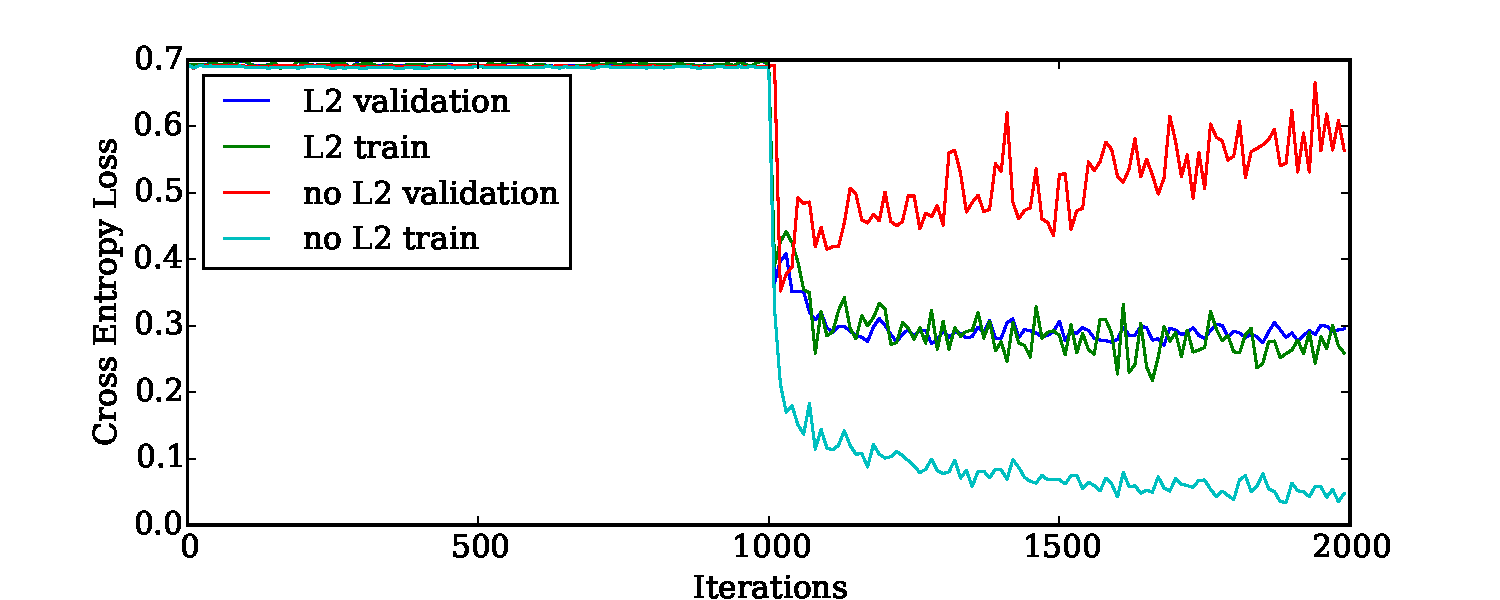
\includegraphics[width =0.8\hsize]{figures/l2.pdf}
    \caption{Plot of the classifier cross entropy loss losses of the two experiments in table \ref{tab:l2_2} }
    \label{fig:l2_1}
    \end{figure}

    \begin{figure}[!h]
    \centering
    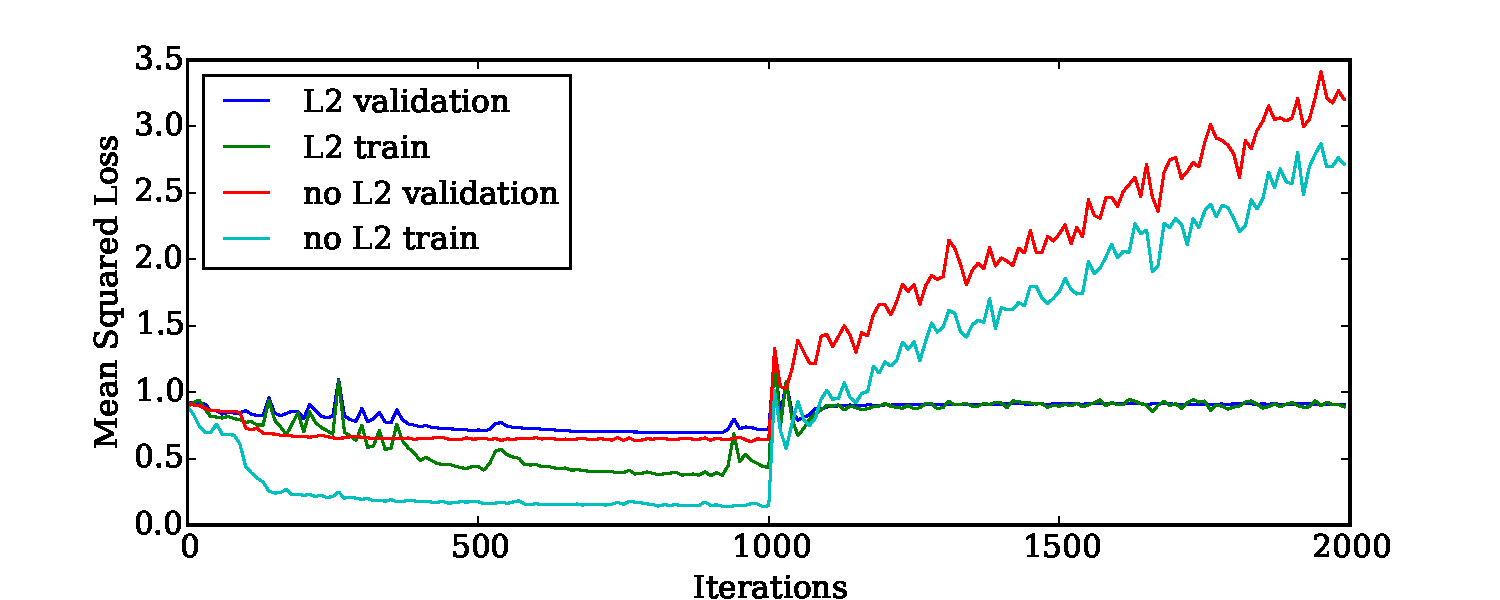
\includegraphics[width =0.8\hsize]{figures/l2_auto.pdf}
    \caption{Plot of the autoencoder mean squared loss of the two experiments in table \ref{tab:l2_2} }
    \label{fig:l2_2}
    \end{figure}

    With these results then, the conclusion is that including a small degree of L2
    Regularisation should be useful for exploring the aims of this project.

    \newpage

  %
  %
  %
  %
  %
  %
  \newpage
  \section{Autoencoder transfer functions}
  In the style of the previous sections, the autoencoder transfer functions are investigated.
  The classifier only situations are included as a baseline from which to compare
  what the autoencoder actually changes. In these experiments, one possible issue is that
  the total amount of classifier and autoencoder training is not constant
  \footnote{In other words the area under the $\alpha(t)$ and $1-\alpha(t)$ curves are not constant between runs.}
  between transfer functions
  and this is something that might be critical for a really precise exposition. However, what is shown here
  instead is if forfeiting some classier training for autoencoder training can give improvements.

  To



  \begin{table}[]
    \footnotesize{
    \centering
    \begin{tabular}{rrrrrrrrrrr}
                         &                      &                      &                                                                              & \multicolumn{1}{r|}{}                                                       & \multicolumn{3}{c|}{Early Model}                                   & \multicolumn{3}{c|}{Final Model}                                   \\ \hline
    i                    & Network              & alpha                & \multirow{2}{*}{\begin{tabular}[c]{@{}r@{}}Total \\ Iterations\end{tabular}} & \multirow{2}{*}{\begin{tabular}[c]{@{}r@{}}Early \\ Iteration\end{tabular}} & ROC                  & F1                   & AE Loss              & ROC                  & F1                   & AE Loss              \\
    \multicolumn{1}{l}{} & \multicolumn{1}{l}{} & \multicolumn{1}{l}{} &                                                                              &                                                                             & \multicolumn{1}{l}{} & \multicolumn{1}{l}{} & \multicolumn{1}{l}{} & \multicolumn{1}{l}{} & \multicolumn{1}{l}{} & \multicolumn{1}{l}{} \\ \hline
    2.1                 & 2                    & step                 & 1500           & 1000    & 0.59  & 0.19 & 0.03  & 0.82 & 0.47 & 0.08  \\
    2.2                  & 2                    & alternate            & 1500           & 1000    & 0.81  & 0.46 & 0.1   & 0.82 & 0.47 & 0.12  \\
    2.3                  & 2                    & constant 0.5         & 1500           & 750     & 0.81  & 0.48 & 0.03  & 0.8  & 0.46 & 0.03  \\
    2.4                  & 2                    & sigmoid              & 1500           & 1000    & 0.8   & 0.46 & 0.03  & 0.79 & 0.46 & 0.03  \\
    2.5                  & 2                    & constant 0.0         & 1500           & 1000    & 0.8   & 0.47 & 0.56  & 0.79 & 0.46 & 0.64  \\
    2.6                  & 2                    & polynomial           & 1500           & 750     & 0.79  & 0.46 & 0.03  & 0.77 & 0.44 & 0.03  \\
    \hline
    3.1                  & 3                    & step                 & 1500           & 1000    & 0.38  & 0.19 & 0.03  & 0.81 & 0.45 & 0.18  \\
    3.2                  & 3                    & constant 0.5         & 1500           & 750     & 0.81  & 0.46 & 0.03  & 0.81 & 0.46 & 0.03  \\
    3.3                  & 3                    & sigmoid              & 1500           & 1000    & 0.8   & 0.46 & 0.03  & 0.8  & 0.44 & 0.04  \\
    3.4                  & 3                    & polynomial           & 1500           & 750     & 0.78  & 0.45 & 0.02  & 0.79 & 0.44 & 0.03  \\
    3.5                  & 3                    & constant 0.0         & 1500           & 1000    & 0.81  & 0.43 & 2.38  & 0.79 & 0.42 & 2.61  \\
    3.6                  & 3                    & alternate            & 1500           & 1000    & 0.69  & 0.32 & 0.1   & 0.77 & 0.37 & 0.23  \\
    \hline
    4.1                  & 4                    & constant 0.0         & 1500           & 1000    & 0.78  & 0.38 & 16.31 & 0.78 & 0.39 & 14.5  \\
    4.2                  & 4                    & step                 & 1500           & 1000    & 0.42  & 0.19 & 0.03  & 0.77 & 0.4  & 0.7   \\
    4.3                  & 4                    & constant 0.5         & 1500           & 750     & 0.73  & 0.33 & 0.03  & 0.75 & 0.36 & 0.03  \\
    4.4                  & 4                    & sigmoid              & 1500           & 1000    & 0.74  & 0.36 & 0.03  & 0.74 & 0.36 & 0.03  \\
    4.5                  & 4                    & polynomial           & 1500           & 750     & 0.52  & 0.21 & 0.09  & 0.67 & 0.3  & 0.04  \\
    4.6                  & 4                    & alternate            & 1500           & 1000    & 0.6   & 0.26 & 0.06  & 0.61 & 0.27 & 0.07  \\
    \hline
    \end{tabular}
    }
    \caption{A comparison of the the autoencoder transfer functions with 0.8 dropout and local contrast normalisation layers (one for network 2 and two for networks 3 \& 4).
    {\bf Experimental Configuration:} see caption for table \ref{tab:sharedweights}.} \label{tab:auto_final_1}
  \end{table}

    The first thing to note from the results in table \ref{tab:auto_final_1} is that
    the constant 0.0 experiments leave the autoencoder in a particularly bad state,
    getting worse with the size of the network. Then there is the observation that
    the ROC scores are fairly close, with the F1 scores being almost the same.

    There is no particular evidence that the smoother alpha functions contribute different
    dynamics, as mentioned earlier this would require fixing the total amount of classifier and autoencoder
    training.



    \begin{figure}[!h]
    \centering
    \includegraphics[width =\hsize]{../graphs/losses_2016_08_24_006.pdf}
    \caption{Losses in experiment 5 in table \ref{}}
    \label{fig:auto}
    \end{figure}

    \newpage


    \newpage
    %
    %
    %
    %
    %
    \section{Results from the best performing network}

  % The Four Pillars of Autofaces
  %%%%%%%%%%%%% The variation between images %%%%%%%%%%%%%%%%%%%%%%%%
  %%%%%%%%%%%%% They contain fewer images %%%%%%%%%%%%%%%%%%%%%%%%%%%
  %%%%%%%%%%%%% The possibility for AUs to occur simultaneously %%%%%
  %%%%%%%%%%%%% Non-uniform AU occurrence %%%%%%%%%%%%%%%%%%%%%%%%%%%
\chapter{Discussion}


  \section{Methodology}
    % - organisation of code and data was good, maybe a bit too late in the day
    %   - good to automate comparison
    % - experimentation structure
    % - iterations posed an issue throughout
    % - suffered from overhead of reproducing existing technique, ideal situation would be to start from something state of the art
    % - suffered from non-deterministic computations, should have used a more mature framework. This might have allowed
    %   above issue to be solved
    % - Limited time so couldn't test more structures
    % - Talk about the fact that the direct inversion of functioning classifiers was the wrong approach,
    %   it should have been to apply state of the art autoencoders and turn them into classifiers
    % - Maybe these classifiers are too big for the purpose.

    This section discusses some of the problems encountered and solutions found
    to issues relating to methodology.

    The structures in this report allow for the exploration of a hyperparameter
    space which is very large. Each parameter has complex non-linear interactions with
    others, hence it is difficult to explore all options and configurations.
    This work has explored a small section of this space with the guide of experimentation
    and existing literature.

    Good organisation of code and data allowed for the easy running
    and comparison of experiments which could take up to a day. These were easily transferred
    into the graphs in this report. Automating many of these tasks therefore seems worthwhile,
    as once the initial overhead of implementation and testing is passed, they encourage experimentation.

    \subsection{Validity of results}

    \begin{itemize}
      \item \textit{Training iterations: }
        The number of iterations used to train a model posed a challenge. Different networks
        and different configurations all need a different number of iterations to produce their
        best possible model. The approach of this work was to fix the number of iterations
        and use the fact that larger models need more iterations to their disadvantage.
        It seems this did not cause a problem, because overfitting was not massively detrimental to the final score, each network could recieve enough iterations to converge.
      \item \textit{Overhead in reproducing state of the art:}
        There was an overhead in trying to reproduce existing work in the literature
        and only then to implement something new. It would have potentially been easier
        to start from an existing state of the art model, however none were openly available
        for the exact required application, many existed for other image classification tasks.
        This was avoided because inverting very deep convolutional networks might be difficult
        and not achieve good performance as training such structures is difficult.
        The approach of taking classification networks from the literature and then
        inverting them to create autoencoders was potentially not ideal, as they
        were not designed with this purpose in mind. Advanced techniques to create robust
        autoencoders might have been a better starting point, this is further discussed in future work.
      \item \textit{Non-deterministic computations:}
        The ability to compare networks was reduced by the fact that TensorFlow could
        not perform deterministic computations even when random number generators were
        seeded.
      \item \textit{Visualisation of convolutional layers:}
        This provided a good way to diagnose and understand what the final to networks
        were learning and helped reach more concrete conclusions.
    \end{itemize}
    % This would have posed some issues however, as inverting a very deep network
    % to create an autoencoder might not have been feasible.



  \section{Results}
    One of the goals of the project was to find a way to increase the variation
    between images in the DISFA dataset in order to allow improved training of the network.
    As is shown in the results (section \ref{tab:psearch}), this is the variable that has
    the greatest effect on classification and autoencoding performance.

    Joint classification of AUs was tackled by proposing the Binary Softmax layer,
    which proved to perform better than the other available solutions.

    The results show that there are cases where both the autoencoder
    and classifier can retain their functionality,
    this is shown in the L2 Regularisation section
    and when both objectives were trained
    equally with constant balance. However there is little evidence that the autoencoder structure which was used
    helps classification. This is most likely because the autoencoder failed to learn enough features.



  \section{Future Work}





    \begin{itemize}
      \item \textit{Larger fully connected models} - Instead of using convolutional networks, the DISFA dataset might have been
                                                     modelled well with just fully connected layers and regularisation techinques.
                                                     This was ignored as the literature mainly used convolutional layers, but might hold
                                                     interesting insights, in particular when combined with the proposed autoencoder classifier structure.
      \item \textit{Start from autoencoders:} -
            Instead of starting from classification structures, state of the art autoencoders
            should be the starting point. These could include the follow techniques stacked architectures\cite{Zhou2014}, denoising architectures\cite{stacks,Vincent2008a} or variational autoencoders\cite{Kingma2013}.
      \item \textit{Improved visualisation of autoencoder features:} As in \cite{Khorrami2015} the maximal excitation for different neurons in convolutional layers
              could be found in order to gain greater insight into what features are being extracted.
      \item \textit{  Artificially increasing the size of the training set:}
            this would allow both the classifier and autoencoder to learn more
            general features. Some methods for doing this are as follows:

            \begin{itemize}
              \item Appyling random transformations to the input image (crops, displacements, etc.)
              \item Training the autoencoder with other datasets
              \item Including high intensity AU examples more often
            \end{itemize}
      \item \textit{ Perform a cross validatation:} this would allow the comparison of the results to the literature.
      \item \textit{ Incorporating temporal information:} facial expressions depend on context
            and are not of constant intensity in time. This information could be incorporated into
            a recurrent neural network structure as in \cite{Jaiswal2016}
    \end{itemize}

\chapter{Conclusion}
  The results have not shown that an autoencoder, in our particular setting,
  gives significant improvements to classification performance. However it has
  explored how preprocessing techniques and various neural network structures
  interact, showing that with small datasets such as DISFA other considerations
  are also important. An unconventional part of this work, given the
  excitement in the field of deep learning is that the smaller networks
  perform better. This is most probably due to the fact that the input data
  was too homogeneous and that the task of detecting AUs is difficult, in
  particular in the way the problem was set up where even intensity one AUs
  (barely visible to humans and related to context) were included as a
  positive example. The method of per subject mean face normalisation was
  found to out perform other preprocessing methods conclusively and the
  classifier achieved competitive results on the DISFA dataset. Lastly the Binary Softmax
  classifier proved to be a useful structure for jointly classifying AUs, giving a maximum average classification ROC of 0.83.

\chapter{Conclusion}
maximal badness

\appendix
\chapter{Networks} \label{appendix1}
\section*{Network 1} \label{net:0}

\begin{table}[h!]
\centering
{\footnotesize
\begin{tabular}{|lllllllll|}
\hline
\multicolumn{1}{|l|}{Element} & Type     & \multicolumn{1}{l|}{Dimensions}                     & Type     & \multicolumn{1}{l|}{Dimensions}  \\ \hline
\multicolumn{1}{|l|}{x}       &          & \multicolumn{1}{l|}{$47\times47\times1$}            &          & \multicolumn{1}{l|}{}        \\ \hline
\multicolumn{1}{|l|}{$L_3$}   & fc       & \multicolumn{1}{l|}{$2209\times14$}              & Binary Softmax & \multicolumn{1}{l|}{$3000\times2\times12$}        \\
\multicolumn{1}{|l|}{$y_4$}   & dropout  & \multicolumn{1}{l|}{$14$}                         &          & \multicolumn{1}{l|}{$24$}        \\ \hline
\multicolumn{1}{|l|}{$L_3$}   & fc       & \multicolumn{1}{l|}{$14\times2209$}              &          & \multicolumn{1}{l|}{}        \\
\multicolumn{1}{|l|}{$y_4$}   &          & \multicolumn{1}{l|}{$3000$}                         &          & \multicolumn{1}{l|}{}        \\ \hline
\multicolumn{1}{|l|}{$L_2$}   & resize\& reshape & \multicolumn{1}{l|}{$2$}                    &          & \multicolumn{1}{l|}{}        \\
\multicolumn{1}{|l|}{$y_2$}   &          & \multicolumn{1}{l|}{$43\times43\times 64$}          &          & \multicolumn{1}{l|}{}        \\ \hline
\end{tabular}

\caption{}

}
\end{table}

\section*{Network 2} \label{net:1}

\begin{table}[h!]
\centering
{\footnotesize
\begin{tabular}{|lllllllll|}
\hline
\multicolumn{1}{|l|}{Element} & Type     & \multicolumn{1}{l|}{Dimensions}                     & Type     & \multicolumn{1}{l|}{Dimensions}  \\ \hline
\multicolumn{1}{|l|}{x}       &          & \multicolumn{1}{l|}{$47\times47\times1$}            &          & \multicolumn{1}{l|}{}        \\ \hline
\multicolumn{1}{|l|}{$L_1$}   & conv 1   & \multicolumn{1}{l|}{$5\times 5\times1\times 64$}    &          & \multicolumn{1}{l|}{}\\
\multicolumn{1}{|l|}{$y_1$}   &          & \multicolumn{1}{l|}{$43\times43\times64$}           &          & \multicolumn{1}{l|}{}        \\ \hline
\multicolumn{1}{|l|}{$L_2$}   & max pool & \multicolumn{1}{l|}{$2\times 2$}                    &          & \multicolumn{1}{l|}{}        \\
\multicolumn{1}{|l|}{$y_2$}   &          & \multicolumn{1}{l|}{$22\times22\times 64$}          &          & \multicolumn{1}{l|}{}        \\ \hline
\multicolumn{1}{|l|}{$L_3$}   & fc       & \multicolumn{1}{l|}{$30976\times3000$}              & Binary Softmax & \multicolumn{1}{l|}{$3000\times2\times12$}        \\
\multicolumn{1}{|l|}{$y_3$}   & dropout  & \multicolumn{1}{l|}{$3000$}                         &          & \multicolumn{1}{l|}{$24$}        \\ \hline
\multicolumn{1}{|l|}{$L_4$}   & fc       & \multicolumn{1}{l|}{$3000\times30976$}              &          & \multicolumn{1}{l|}{}        \\
\multicolumn{1}{|l|}{$y_4$}   &          & \multicolumn{1}{l|}{$3000$}                         &          & \multicolumn{1}{l|}{}        \\ \hline
\multicolumn{1}{|l|}{$L_5$}   & resize\& reshape & \multicolumn{1}{l|}{$2$}                    &          & \multicolumn{1}{l|}{}        \\
\multicolumn{1}{|l|}{$y_5$}   &          & \multicolumn{1}{l|}{$43\times43\times 64$}          &          & \multicolumn{1}{l|}{}        \\ \hline
\multicolumn{1}{|l|}{$L_6$}   & deconv 1   & \multicolumn{1}{l|}{$5\times 5\times1\times 64$}    &          & \multicolumn{1}{l|}{}\\
\multicolumn{1}{|l|}{$y_6$}   &          & \multicolumn{1}{l|}{$47\times47\times1$}           &          & \multicolumn{1}{l|}{}        \\ \hline
\end{tabular}

\caption{} \label{compnet}

}
\end{table}

\section*{Network 3} \label{net:2}
\section*{Network 4} \label{net:2}
\section*{ResNet 1} \label{net:res1}


%% bibliography
\bibliographystyle{unsrt}
\bibliography{bib/autofaces}
\end{document}
